\documentclass[]{book}
\usepackage{lmodern}
\usepackage{amssymb,amsmath}
\usepackage{ifxetex,ifluatex}
\usepackage{fixltx2e} % provides \textsubscript
\ifnum 0\ifxetex 1\fi\ifluatex 1\fi=0 % if pdftex
  \usepackage[T1]{fontenc}
  \usepackage[utf8]{inputenc}
\else % if luatex or xelatex
  \ifxetex
    \usepackage{mathspec}
  \else
    \usepackage{fontspec}
  \fi
  \defaultfontfeatures{Ligatures=TeX,Scale=MatchLowercase}
\fi
% use upquote if available, for straight quotes in verbatim environments
\IfFileExists{upquote.sty}{\usepackage{upquote}}{}
% use microtype if available
\IfFileExists{microtype.sty}{%
\usepackage{microtype}
\UseMicrotypeSet[protrusion]{basicmath} % disable protrusion for tt fonts
}{}
\usepackage{hyperref}
\hypersetup{unicode=true,
            pdftitle={Using R at Grattan Institute},
            pdfauthor={Will Mackey and Matt Cowgill},
            pdfborder={0 0 0},
            breaklinks=true}
\urlstyle{same}  % don't use monospace font for urls
\usepackage{natbib}
\bibliographystyle{apalike}
\usepackage{color}
\usepackage{fancyvrb}
\newcommand{\VerbBar}{|}
\newcommand{\VERB}{\Verb[commandchars=\\\{\}]}
\DefineVerbatimEnvironment{Highlighting}{Verbatim}{commandchars=\\\{\}}
% Add ',fontsize=\small' for more characters per line
\usepackage{framed}
\definecolor{shadecolor}{RGB}{248,248,248}
\newenvironment{Shaded}{\begin{snugshade}}{\end{snugshade}}
\newcommand{\AlertTok}[1]{\textcolor[rgb]{0.94,0.16,0.16}{#1}}
\newcommand{\AnnotationTok}[1]{\textcolor[rgb]{0.56,0.35,0.01}{\textbf{\textit{#1}}}}
\newcommand{\AttributeTok}[1]{\textcolor[rgb]{0.77,0.63,0.00}{#1}}
\newcommand{\BaseNTok}[1]{\textcolor[rgb]{0.00,0.00,0.81}{#1}}
\newcommand{\BuiltInTok}[1]{#1}
\newcommand{\CharTok}[1]{\textcolor[rgb]{0.31,0.60,0.02}{#1}}
\newcommand{\CommentTok}[1]{\textcolor[rgb]{0.56,0.35,0.01}{\textit{#1}}}
\newcommand{\CommentVarTok}[1]{\textcolor[rgb]{0.56,0.35,0.01}{\textbf{\textit{#1}}}}
\newcommand{\ConstantTok}[1]{\textcolor[rgb]{0.00,0.00,0.00}{#1}}
\newcommand{\ControlFlowTok}[1]{\textcolor[rgb]{0.13,0.29,0.53}{\textbf{#1}}}
\newcommand{\DataTypeTok}[1]{\textcolor[rgb]{0.13,0.29,0.53}{#1}}
\newcommand{\DecValTok}[1]{\textcolor[rgb]{0.00,0.00,0.81}{#1}}
\newcommand{\DocumentationTok}[1]{\textcolor[rgb]{0.56,0.35,0.01}{\textbf{\textit{#1}}}}
\newcommand{\ErrorTok}[1]{\textcolor[rgb]{0.64,0.00,0.00}{\textbf{#1}}}
\newcommand{\ExtensionTok}[1]{#1}
\newcommand{\FloatTok}[1]{\textcolor[rgb]{0.00,0.00,0.81}{#1}}
\newcommand{\FunctionTok}[1]{\textcolor[rgb]{0.00,0.00,0.00}{#1}}
\newcommand{\ImportTok}[1]{#1}
\newcommand{\InformationTok}[1]{\textcolor[rgb]{0.56,0.35,0.01}{\textbf{\textit{#1}}}}
\newcommand{\KeywordTok}[1]{\textcolor[rgb]{0.13,0.29,0.53}{\textbf{#1}}}
\newcommand{\NormalTok}[1]{#1}
\newcommand{\OperatorTok}[1]{\textcolor[rgb]{0.81,0.36,0.00}{\textbf{#1}}}
\newcommand{\OtherTok}[1]{\textcolor[rgb]{0.56,0.35,0.01}{#1}}
\newcommand{\PreprocessorTok}[1]{\textcolor[rgb]{0.56,0.35,0.01}{\textit{#1}}}
\newcommand{\RegionMarkerTok}[1]{#1}
\newcommand{\SpecialCharTok}[1]{\textcolor[rgb]{0.00,0.00,0.00}{#1}}
\newcommand{\SpecialStringTok}[1]{\textcolor[rgb]{0.31,0.60,0.02}{#1}}
\newcommand{\StringTok}[1]{\textcolor[rgb]{0.31,0.60,0.02}{#1}}
\newcommand{\VariableTok}[1]{\textcolor[rgb]{0.00,0.00,0.00}{#1}}
\newcommand{\VerbatimStringTok}[1]{\textcolor[rgb]{0.31,0.60,0.02}{#1}}
\newcommand{\WarningTok}[1]{\textcolor[rgb]{0.56,0.35,0.01}{\textbf{\textit{#1}}}}
\usepackage{longtable,booktabs}
\usepackage{graphicx,grffile}
\makeatletter
\def\maxwidth{\ifdim\Gin@nat@width>\linewidth\linewidth\else\Gin@nat@width\fi}
\def\maxheight{\ifdim\Gin@nat@height>\textheight\textheight\else\Gin@nat@height\fi}
\makeatother
% Scale images if necessary, so that they will not overflow the page
% margins by default, and it is still possible to overwrite the defaults
% using explicit options in \includegraphics[width, height, ...]{}
\setkeys{Gin}{width=\maxwidth,height=\maxheight,keepaspectratio}
\IfFileExists{parskip.sty}{%
\usepackage{parskip}
}{% else
\setlength{\parindent}{0pt}
\setlength{\parskip}{6pt plus 2pt minus 1pt}
}
\setlength{\emergencystretch}{3em}  % prevent overfull lines
\providecommand{\tightlist}{%
  \setlength{\itemsep}{0pt}\setlength{\parskip}{0pt}}
\setcounter{secnumdepth}{5}
% Redefines (sub)paragraphs to behave more like sections
\ifx\paragraph\undefined\else
\let\oldparagraph\paragraph
\renewcommand{\paragraph}[1]{\oldparagraph{#1}\mbox{}}
\fi
\ifx\subparagraph\undefined\else
\let\oldsubparagraph\subparagraph
\renewcommand{\subparagraph}[1]{\oldsubparagraph{#1}\mbox{}}
\fi

%%% Use protect on footnotes to avoid problems with footnotes in titles
\let\rmarkdownfootnote\footnote%
\def\footnote{\protect\rmarkdownfootnote}

%%% Change title format to be more compact
\usepackage{titling}

% Create subtitle command for use in maketitle
\providecommand{\subtitle}[1]{
  \posttitle{
    \begin{center}\large#1\end{center}
    }
}

\setlength{\droptitle}{-2em}

  \title{Using R at Grattan Institute}
    \pretitle{\vspace{\droptitle}\centering\huge}
  \posttitle{\par}
    \author{Will Mackey and Matt Cowgill}
    \preauthor{\centering\large\emph}
  \postauthor{\par}
      \predate{\centering\large\emph}
  \postdate{\par}
    \date{2019-09-15}

\usepackage{booktabs}
\usepackage{amsthm}
\makeatletter
\def\thm@space@setup{%
  \thm@preskip=8pt plus 2pt minus 4pt
  \thm@postskip=\thm@preskip
}
\makeatother

\begin{document}
\maketitle

{
\setcounter{tocdepth}{1}
\tableofcontents
}
\hypertarget{welcome}{%
\chapter*{Welcome}\label{welcome}}
\addcontentsline{toc}{chapter}{Welcome}

This guide is designed for everyone who uses - or would like to use - R at Grattan Institute.

It does two main things:

\begin{enumerate}
\def\labelenumi{\arabic{enumi}.}
\tightlist
\item
  Shows you how to use R to complete common analytical tasks you'll face at Grattan.
\item
  Sets out some guidelines and good practices when using R at Grattan.
\end{enumerate}

As a guide to using R, this website is helpful but incomplete. We can't possibly cover - or anticipate - all the skills you might need to know. If you make it to the end of this guide and want to learn more, start by reading \href{https://r4ds.had.co.nz}{R for Data Science} by Hadley Wickham and Garrett Grolemund. It's free.

Any complaints or comments about this guide can be sent to Will or Matt, respectively.

This site was written in R with RMarkdown and the \href{https://bookdown.org}{bookdown} package.

\hypertarget{introduction-to-r}{%
\chapter{Introduction to R}\label{introduction-to-r}}

Most people reading this guide will know what R is. But if you don't - that's OK!

If you have used R before and are comfortable enough with it, you might want to skip to the next page. This page is intended for people who are unfamiliar with R.

\hypertarget{what-is-r}{%
\section{What is R?}\label{what-is-r}}

R is a programming language that is designed by and for statisticians, data scientists, and other people who work with data. It's free - you can download R at no charge. It's also open source - you can view and (if you're game) modify the code that underlies the R language. R is available for all major computing platforms including Windows, macOS, and Linux.

R has a lot in common with other statistical software like SAS, Stata, SPSS or Eviews. You can use those software packages to read data, manipulate it, generate summary statistics, estimate models, and so on. You can use R for all those things and more.

You interact with R by writing code. This is a little different to Stata or SPSS, which allow you to do at least part of your analyses by clicking on menus and buttons. This means the initial learning curve for R can be a little steeper than for something like SPSS, but there are great benefits to a code-based approach to data analysis (\protect\hyperlink{why-script}{see the next page for more on this}).

R also has a fair bit of overlap with general purpose programming languages like Python. But R is more focused on the sort of tasks that statisticians, data scientists, and academic researchers do.

R is quite old, having been first released publicly in 1995, but it's also growing and changing rapidly. A lot of developments in R come in the form of new add-on pieces of software - known as `packages' - that extend R's functionality in some way. We cover packages more \protect\hyperlink{packages}{later in this page}.

When you open R itself, you're confronted with a few disclaimers and a command prompt, similar in appearance to the Terminal on macOS or command prompt in Windows.

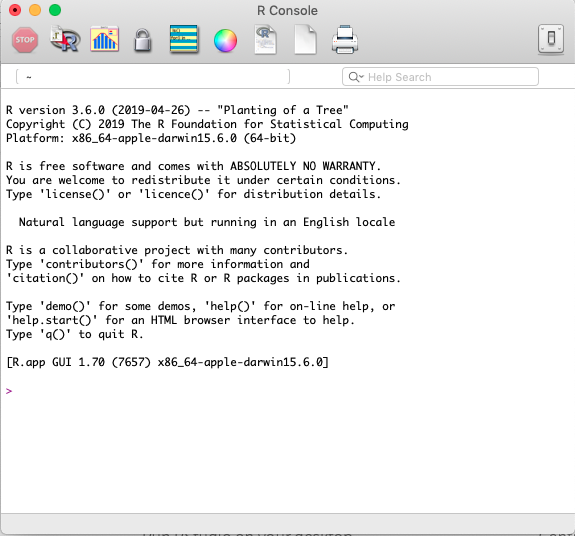
\includegraphics[width=7.99in]{atlas/r_screenshot}

This might look a bit intimidating, but you'll almost never open R directly and interact with it in that way.

To analyse data with R, you will typically write out a text file containing code. This file - which we'll call a script - should be able to be read and executed by R from start to finish. The easiest way to write your code, run your script, and generate your outputs (whether that's a chart, a document, or a set of model results) is to use RStudio.

\hypertarget{what-is-rstudio}{%
\section{What is RStudio?}\label{what-is-rstudio}}

RStudio is another piece of free software you can download and run on your computer.\footnote{RStudio is, somewhat confusingly, a product made by a company called RStudio. Although the RStudio desktop software is free, RStudio makes money by charging for other services, like running R in the cloud. When we refer to RStudio, we're referring to the desktop software unless we make it clear that we mean the company.} Like R itself, RStudio is available for Windows, macOS and Linux. In programmer jargon, RStudio is an ``integrated development environment'' or IDE. Translated to English, this means RStudio has a range of tools that help you work with R. It has a text editor for you to write R scripts, an R `console' to interact directly with the language, and panes that let you see the objects you have stored in memory and any graphs you've created, among other things.

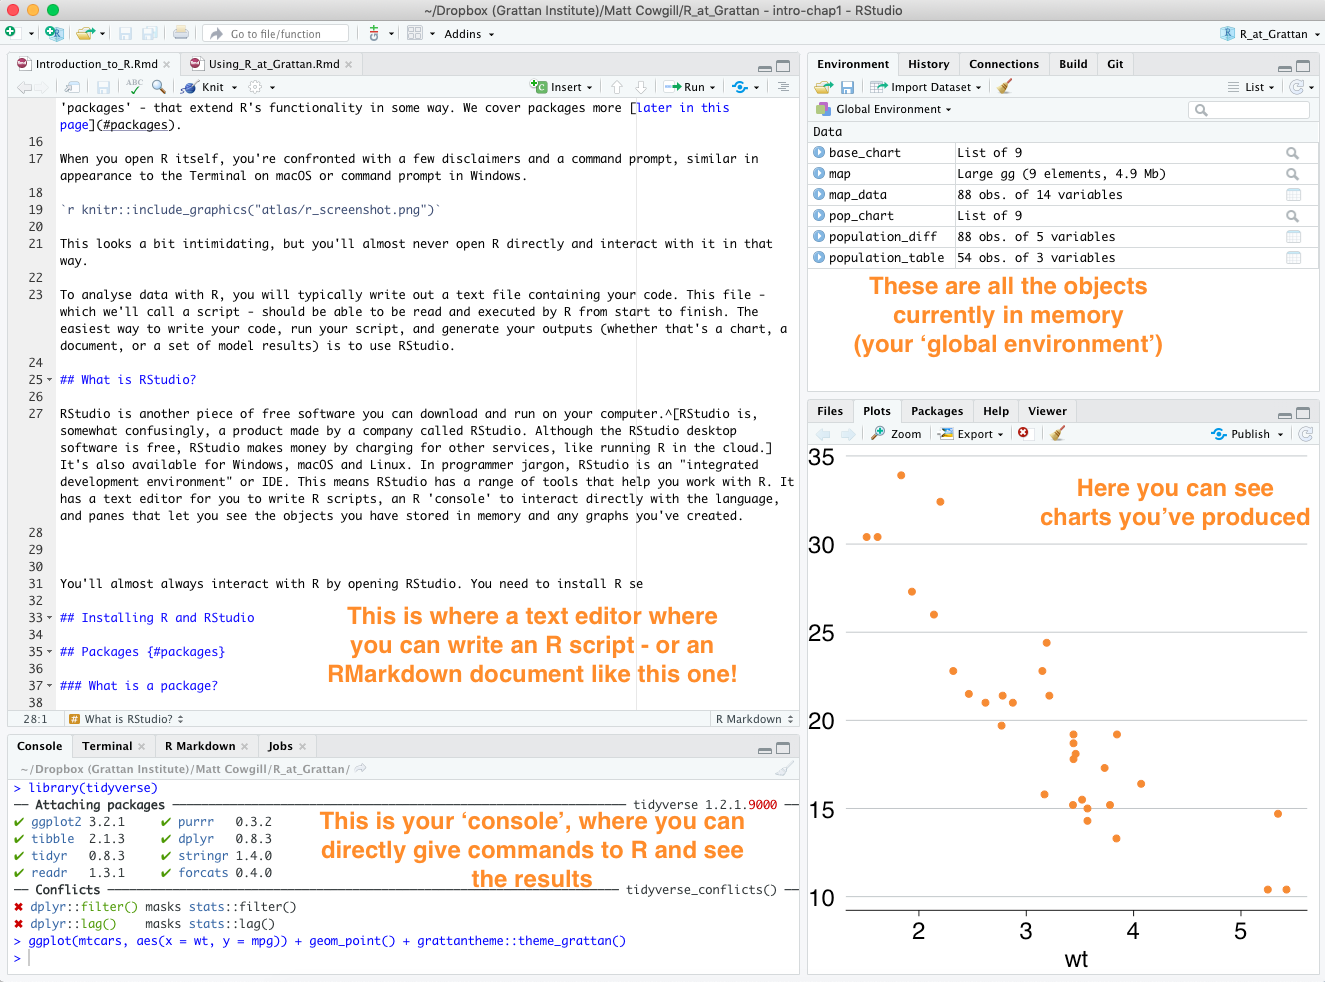
\includegraphics[width=18.4in]{atlas/rstudio_screenshot}

You'll almost always interact with R by opening RStudio.

\hypertarget{installing-r-and-rstudio}{%
\section{Installing R and RStudio}\label{installing-r-and-rstudio}}

Although you'll usually work with R by opening RStudio, you need to install both R and RStudio separately.

Install R by going to \href{https://cran.r-project.org}{CRAN}, the Comprehensive R Archive Network. CRAN is a community-run website that houses R itself as well as a broad range of R packages.

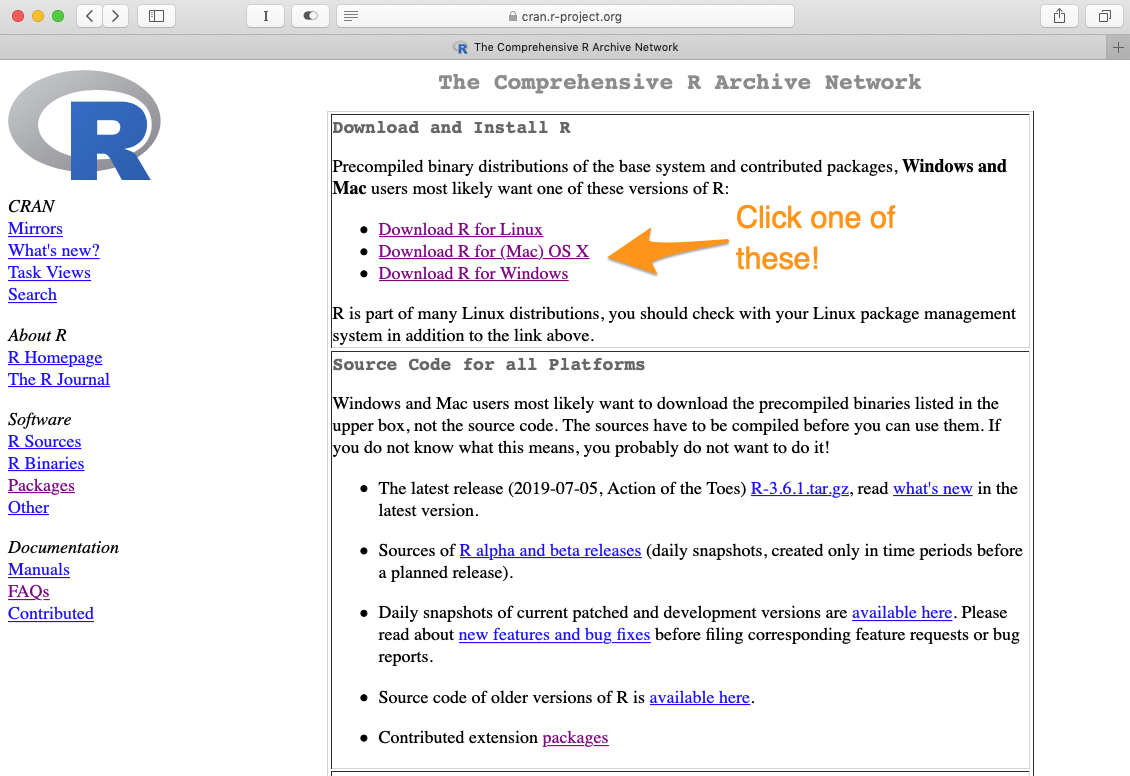
\includegraphics[width=15.69in]{atlas/r_cran}

You want to download the latest base R release, as a `binary'. Don't worry, you don't need to know what a binary is.

For macOS, the page will look like this:

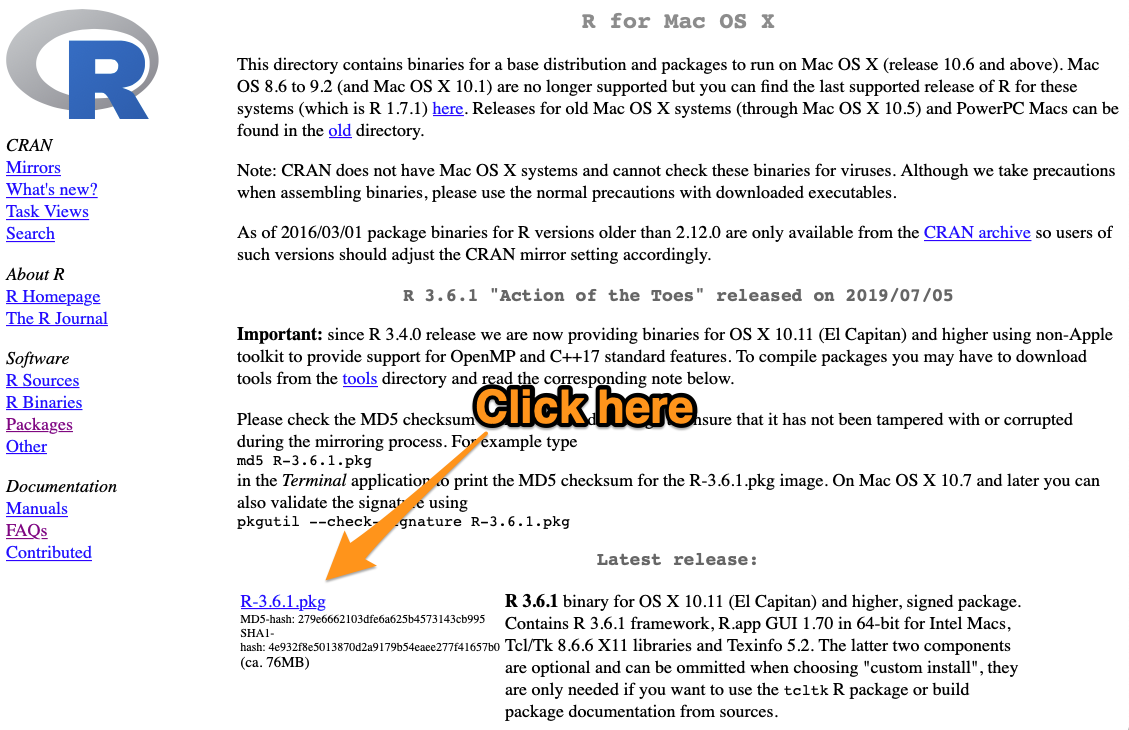
\includegraphics[width=15.68in]{atlas/r_cran_macos}

For Windows, you'll need to click on the `base' version, and then click again to start the download.

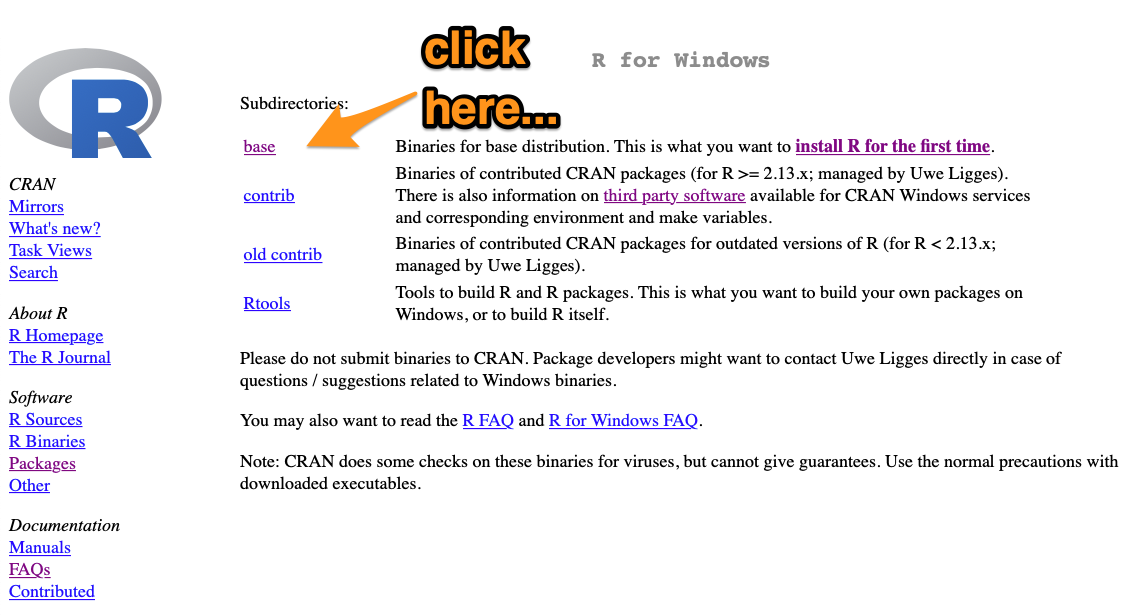
\includegraphics[width=15.69in]{atlas/r_cran_windows_1}
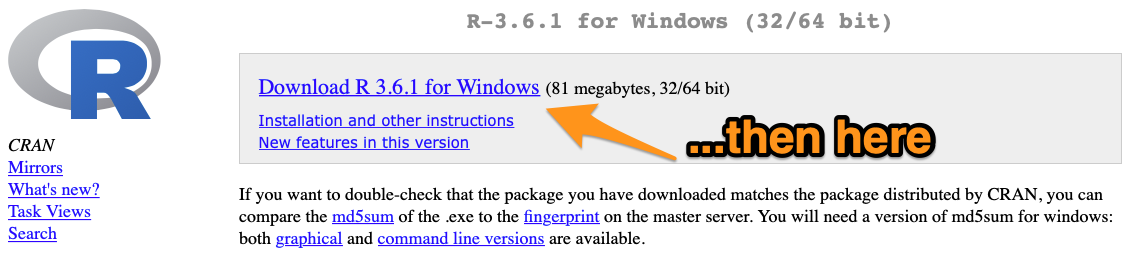
\includegraphics[width=15.67in]{atlas/r_cran_windows_2}

Once you've installed R, you'll need to install RStudio. Go to the \href{https://www.rstudio.com/products/rstudio/download/\#download}{RStudio website and install the latest version} of RStudio Desktop (open source license).

Once they're both installed, get started by opening RStudio.

\hypertarget{packages}{%
\section{Packages}\label{packages}}

R comes with a lot of functions - commands - built in to do a broad range of tasks. You could, if you really wanted, import a dataset, clean it up, estimate a model, and make a plot all using the functions that come with R - known as `base R'\footnote{Technically some of the `built-in' functions are part of packages, like the \texttt{tools}, \texttt{utils} and \texttt{stats} packages that come with R. We'll refer to all these as base R.}.

But a lot of our work at Grattan uses add-on software to base R, known as `packages'. Some packages, like the popular `dplyr', make it quicker and/or easier to do tasks that you could otherwise do in base R. Other packages expand the possibilities of what R can do - like fitting a machine learning model, for example.

Like R itself, packages are free and open source. You can install them from within RStudio.

At Grattan, we make heavy use of a set of related packages known collectively as the \texttt{tidyverse}. We'll cover this more in a later chapter.

\hypertarget{installing-packages}{%
\subsection{Installing packages}\label{installing-packages}}

You'll typically install packages using the console in RStudio. That's the part of the window that, by default, sits in the bottom-left corner of the screen.

In our work at Grattan, we use packages from two different source: CRAN and Github. The main difference you need to know about is that we use different commands to install packages from these two sources.

To install a package from CRAN, we use the command \texttt{install.packages()}.

For example, this code will install the \texttt{ggplot2} package from CRAN:

\begin{Shaded}
\begin{Highlighting}[]
\KeywordTok{install.packages}\NormalTok{(}\StringTok{"ggplot2"}\NormalTok{)}
\end{Highlighting}
\end{Shaded}

The easiest way to install a package from Github is to use the function \texttt{install\_github()}. Unfortunately, this function doesn't come with base R. The \texttt{install\_github()} function is part of the \texttt{remotes} package. To use it, we first need to install \texttt{remotes} from CRAN:

\begin{Shaded}
\begin{Highlighting}[]
\KeywordTok{install.packages}\NormalTok{(}\StringTok{"remotes"}\NormalTok{)}
\end{Highlighting}
\end{Shaded}

Now we can install packages from Github using the \texttt{install\_github()} function from the \texttt{remotes} package. For example, here's how we would install the Grattan ggplot2 theme, which we'll discuss later in this website:

\begin{Shaded}
\begin{Highlighting}[]
\NormalTok{remotes}\OperatorTok{::}\KeywordTok{install_github}\NormalTok{(}\StringTok{"mattcowgill/grattantheme"}\NormalTok{, }\DataTypeTok{dependencies =} \OtherTok{TRUE}\NormalTok{, }\DataTypeTok{upgrade =} \StringTok{"always"}\NormalTok{)}
\end{Highlighting}
\end{Shaded}

\hypertarget{using-packages}{%
\subsection{Using packages}\label{using-packages}}

Before using a function that comes from a package, as opposed to base R, you need to tell R where to look for the function. There are two main ways to do that.

We can either load (aka `attach') the package by using the \texttt{library()} function. We typically do this at the top of a script.

\begin{Shaded}
\begin{Highlighting}[]
\KeywordTok{library}\NormalTok{(remotes)}

\CommentTok{# Now that the `remotes` package is loaded, we can use its `install_github()` function:}

\KeywordTok{install_github}\NormalTok{(}\StringTok{"mattcowgill/grattantheme"}\NormalTok{)}
\end{Highlighting}
\end{Shaded}

Or, we can use two colons - \texttt{::} - to tell R to use an individual function from a package without loading it:

\begin{Shaded}
\begin{Highlighting}[]
\NormalTok{remotes}\OperatorTok{::}\KeywordTok{install_github}\NormalTok{(}\StringTok{"mattcowgill/grattantheme"}\NormalTok{)}
\end{Highlighting}
\end{Shaded}

It usually makes sense to load a package with \texttt{library()}, unless you only need to use one of its function once or twice. There's no harm to using the \texttt{::} operator even if you have already loaded a package with \texttt{library()}. This can remove ambiguity both for R and for humans reading your code, particularly if you're using an obscure function - it makes it clearer where the function comes from.

\hypertarget{why-use-r}{%
\chapter{Why use R?}\label{why-use-r}}

We can break this question into two parts:

\begin{enumerate}
\def\labelenumi{\arabic{enumi}.}
\tightlist
\item
  Why use script-based software to analyse data?
\item
  Why use R, specifically?
\end{enumerate}

\hypertarget{why-script}{%
\section{Why use script-based software?}\label{why-script}}

It's important for our analyses to be \textbf{reproducible}. This means that all of the steps that were taken to go from your raw data to your final outputs are clearly set out and can be reproduced if necessary.

Reproducibility is very important for QC, particularly of complex analyses - if it's not clear what you've done, it's hard for someone to check your work. It also makes things easier for you in the future - coming back to an old analysis a few months or years down the track is much easier if it's reproducible.

Script-based analyses are more likely to be reproducible.\footnote{Using a script-based approach doesn't guarantee that your analysis will be truly reproducible. If your work involves some steps that aren't documented in the script - such as data ``cleaning'' in Excel - then it is not fully reproducible.} A script sets out all the steps that were taken from reading in data, to tidying it, to estimating models or summary statistics and generating output.

Analysis that isn't script based, like work done in Excel, is almost never reproducible. It is generally unclear what steps were taken, in which order, to go from the raw data to the output. It isn't even always clear in a spreadsheet what is the `raw data' and what has been modified in some way.

Using scripts makes us less susceptible to the sort of errors \href{https://en.wikipedia.org/wiki/Growth_in_a_Time_of_Debt\#Methodological_flaws}{famously made by the economists Reinhart and Rogoff} in their Excel-based analysis of the effect of public debt on economic growth. It's still possible to make errors in a script-based analysis, but those errors are easier to find when the analysis is more transparent.

Script-based analysis software also allows us to:
* Work with larger data sets;
* Work with data in a broader range of formats;
* Easily combine different data sets;
* Automate tasks and build from previous analyses; and
* Estimate statistical models.

\hypertarget{why-R}{%
\section{Why use R specifically?}\label{why-R}}

Doing reproducible, script-based, research doesn't necessarily involve using R. It's perfectly possible to do reproducible work in Stata or Python (though harder in SPSS, where data is primarily manipulated by clicking things).

We use R specifically because:
* It's free!
* It's open source.
* It's powerful, particularly when it comes to statistics and data science.
* It's flexible.
* It has an active community extending its capabilities all the time and providing support online.
* It is becoming the norm in academic research and common in the corporate world.

Everything you can do in Excel can be done in R.

\hypertarget{organising-projects}{%
\chapter{Organising an R project at Grattan}\label{organising-projects}}

All our work, in R or otherwise, should heed the ``hit by a bus'' rule - if you're not around, colleagues should be able to access, understand, verify, and build on the work you've done.

Organising your analysis in a predictable, consistent way helps to make your work reproducible by others, including yourself in the future. This is really important! If your analysis is messy, you're more likely to make errors, and less likely to spot them. Other people will find it hard to check your analysis and you'll find it harder to return to it down the track.

This page sets out some guidelines for organising your work in R at Grattan. It covers:

\begin{itemize}
\tightlist
\item
  Using RStudio projects and relative filepaths
\item
  Using a consistent subfolder structure
\item
  Naming your scripts and keeping them manageable
\item
  Coding style at Grattan
\end{itemize}

\hypertarget{use-rstudio-projects-not-setwd}{%
\section{\texorpdfstring{Use RStudio projects, not \texttt{setwd()}}{Use RStudio projects, not setwd()}}\label{use-rstudio-projects-not-setwd}}

You'll almost always be reading and/or writing files to disk as part of your analysis in R. To do this, R needs to know where to read files from and save files to. By default, it uses your working directory.

One way to tell R which folder to use as your working directory is using the command \texttt{setwd()}, like \texttt{setwd("\textasciitilde{}/Desktop/some\ random\ folder")} or \texttt{setwd("C:\textbackslash{}Users\textbackslash{}mcowgill\textbackslash{}Documents\textbackslash{}Somerandomfolder")}. \textbf{This is a bad idea!} If anyone - including you - tries to run your script on a different machine, with a different folder structure, it probably won't work. If people can't get past the first line when they're trying to run your script, there's an annoying and unnecessary hurdle to reproducing and checking your analysis.

In the \href{https://www.tidyverse.org/articles/2017/12/workflow-vs-script/}{words of Jenny Bryan}:

\begin{quote}
if the first line of your R script is \texttt{setwd("C:\textbackslash{}Users\textbackslash{}jenny\textbackslash{}path\textbackslash{}that\textbackslash{}only\textbackslash{}I\textbackslash{}have")} I will come into your office and SET YOUR COMPUTER ON FIRE.
\end{quote}

Seems fair.

Creating a `project' in RStudio sets your working directory in a way that's portable across machines. Creating an RStudio project is straightforward: \textbf{click File, then New Project}. You can then choose to start your project in a new directory, or an existing directory. Simple!

\begin{center}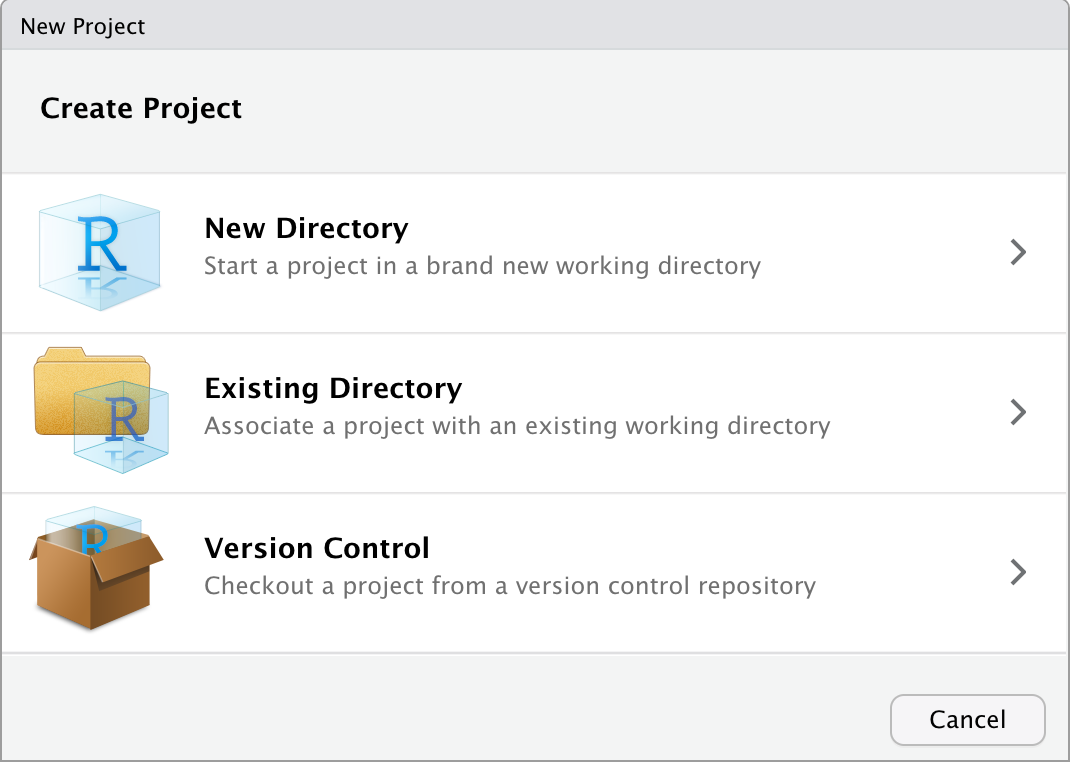
\includegraphics[width=0.66\linewidth]{atlas/rstudio_newproject} \end{center}

RStudio will then create a file with an .Rproj extension in the folder you've chosen. When you want to work in this project, just open the .Rproj file, or click File -\textgreater{} Open project in RStudio. Your working directory will be set to the directory that contains the .Rproj file.

\hypertarget{keep-your-stuff-together}{%
\section{Keep your stuff together}\label{keep-your-stuff-together}}

Your script(s), data, and output should generally all live in the same place. \footnote{This isn't always possible, like when you're working with restricted-access microdata. But unless there's a really good reason why you can't keep your data together with the rest of your work, you should do it.} That place should be the folder that contains the .Rproj file that was created when you created an RStudio project, and subfolders of that folder.

Don't just put everything in your project folder itself. This can get really overwhelming and confusing, particularly for anyone trying to understand and check your work. Instead, separate your code, your source data, and your output into subfolders.

A good structure is to have a subfolder for:

\begin{itemize}
\tightlist
\item
  your code - called `R'
\item
  your source data - called `data'
\item
  your graphs - called `atlas', like in our LaTeX projects
\item
  your non-graph output, like formatted tables, called `output'
\end{itemize}

Sometimes your data folder might have subfolders - `raw' for data that you've done nothing to, and `clean' for data you've modified in some way.\footnote{Other folder structures are OK and might make more sense for your project. The important thing is to \textbf{have} a folder structure, and to use a structure that is easily comprehensible to anyone else looking at your analysis.}

\hypertarget{include-a-readme-file}{%
\section{Include a README file}\label{include-a-readme-file}}

Your analysis workflow might seem completely obvious to you. Let's say that in one script you load raw ABS microdata, run a particular script to clean it up, save the cleaned data somewhere, then load that cleaned data in a second script to produce a summary table, then use a third script to produce a graph based on the summary table. Easy!

Except that might not seem easy or self-explanatory to anyone who comes along and tries to figure out how your analysis works, including you in the future.

Make things easier by including a short text file - called README - in the project folder. This should explain the purpose of the project, the key files, and (if it isn't clear) the order in which they should be run. If you got the data from somewhere non-obvious, explain that in the README file.

\hypertarget{use-relative-filepaths}{%
\section{Use relative filepaths}\label{use-relative-filepaths}}

When you read or write files with R, don't use filepaths that are specific to your machine. For one thing, these machine-specific filepaths will fail when someone else tries to run your script. For another, they're super annoying! Who wants to type out a full filepath everytime you load or save a file?

\textbf{Bad}

\begin{Shaded}
\begin{Highlighting}[]
\NormalTok{hes <-}\StringTok{ }\KeywordTok{read_csv}\NormalTok{(}\StringTok{"/Users/mcowgill/Desktop/hes1516.csv"}\NormalTok{)}
\NormalTok{hes <-}\StringTok{ }\KeywordTok{read_csb}\NormalTok{(}\StringTok{"C:\textbackslash{}Users\textbackslash{}mcowgill\textbackslash{}Desktop\textbackslash{}hes1516.csv"}\NormalTok{)}
\KeywordTok{grattan_save}\NormalTok{(}\StringTok{"/Users/mcowgill/Desktop/images/expenditure_by_income.pdf"}\NormalTok{)}
\end{Highlighting}
\end{Shaded}

Instead, use relative filepaths. These are filepaths that are relative (hence the name) to your project folder, which you set by creating an RStudio project.

\textbf{Good}

\begin{Shaded}
\begin{Highlighting}[]
\NormalTok{hes <-}\StringTok{ }\KeywordTok{read_csv}\NormalTok{(}\StringTok{"data/HES/hes1516.csv"}\NormalTok{)}
\KeywordTok{grattan_save}\NormalTok{(}\StringTok{"atlas/expenditure_by_income.pdf"}\NormalTok{)}
\end{Highlighting}
\end{Shaded}

The first example above tells R to look in the `data' subdirectory of your project folder, and then the `HES' subdirectory of `data', to find the `hes1516.csv' file. This file path isn't specific to your machine, so your code is more shareable this way.

\hypertarget{manageable}{%
\section{Keep your scripts manageable}\label{manageable}}

Unless your project is very simple, it's probably not a good idea to put all your work into one R script. Instead, break your analysis into discrete pieces and put each piece in its own file. Number the files to make it clear what order they're supposed to be run in.

Here's a useful structure:

\begin{itemize}
\tightlist
\item
  01\_import.R
\item
  02\_tidy.R
\item
  03\_model.R
\item
  04\_visualise.R
\end{itemize}

It should be clear what each script is trying to do. Use meaningful filenames that clearly indicate the overarching purpose of the script. Use comments to explain why you're doing things!

\hypertarget{omit-needless-code}{%
\section{Omit needless code}\label{omit-needless-code}}

Don't retain code that ultimately didn't lead anywhere. If you produced a graph that ended up not being used, don't keep the code in your script - if you want to save it, move it to a subfolder named `archive' or similar. Your code should include the steps needed to go from your raw data to your output - and not extraneous steps. If you ask someone to QC your work, they shouldn't have to wade through 1000 lines of code just to find the 200 lines that are actually required to produce your output.

When you're doing data analysis, you'll often give R interactive commands to help you understand what your data looks like. For example, you might view a dataframe with \texttt{View(mydf)} or \texttt{str(mydf)}. This is fine, and often necessary, when you're doing your analysis. \textbf{Don't keep these commands in your script}. These type of commands should usually be entered straight into the R console, not in a script.

\hypertarget{rules_9a_final_final_mc}{%
\section{Rules\_9a\_FINAL\_FINAL\_MC}\label{rules_9a_final_final_mc}}

We're all familiar with this hellish scenario: you do some work in a Word document (shudder, shudder, etc.), email it to a colleague, the colleague edits it and sends it back with a tweaked filename, like \texttt{cool\_word\_doc\_002.docx}. Try to avoid replicating this nightmare in R.

\textbf{Don't} create multiple versions of the same script (like \texttt{analysis\_FINAL\_002\_MC.R} and \texttt{analysis\_FINALFINAL\_003\_MC\_WM.R}.) If you do end up with multiple versions, put everything other than the latest version in a subfolder of your ``R'' folder, called ``R/archive''. To avoid a horrible mess of \texttt{analysis\_FINAL\_002.R} type documents cluttering up your folder, consider using \protect\hyperlink{version-control}{Git for version control}.

\hypertarget{grattan-coding-style}{%
\chapter{Grattan coding style}\label{grattan-coding-style}}

This Grattan style guide is a condensed and lightly adapted version of the Hadley Wickham's \texttt{tidyverse} style guide, found at \url{https://style.tidyverse.org/}.

The benefits of a common coding style are well explained \href{http://r-pkgs.had.co.nz/style.html}{by Hadley}:

\begin{quote}
Good style is important because while your code only has one author, it'll usually have multiple readers. This is especially true when you're writing code with others. In that case, it's a good idea to agree on a common style up-front.
\end{quote}

Below we describe the \textbf{key} code-style elements, without being too tedious about it all. There are many elements of coding style we don't cover in this guide; if you're unsure about anything, \href{https://style.tidyverse.org/}{consult the \texttt{tidyverse} guide}.

You should also see the \protect\hyperlink{organising-projects}{Using R at Grattan} page for guidelines about setting up projects.

\hypertarget{script-preamble}{%
\section{Script preamble}\label{script-preamble}}

Describe what your script does in the first few lines using comments or within an RMarkdown document.

\textbf{Good}

\begin{Shaded}
\begin{Highlighting}[]
\CommentTok{# This script reads ABS data downloaded from TableBuilder and combines into a single data object containing post-secondary education levels by age and gender by SA3. }
\end{Highlighting}
\end{Shaded}

\textbf{Bad}

\begin{Shaded}
\begin{Highlighting}[]
\CommentTok{# make ABS ed data graph}
\end{Highlighting}
\end{Shaded}

If it's hard to concisely describe what your script does in a comment, that might be a sign that your script does too many things. Consider breaking your analysis into a series of scripts. See \protect\hyperlink{organising-projects}{Organising R Projects at Grattan} for more.

\hypertarget{comments}{%
\section{Comments}\label{comments}}

Comments are necessary where the code \emph{alone} doesn't tell the full story. This is important when groups are coded with numbers rather than character strings:

\textbf{Necessary to comment}

\begin{Shaded}
\begin{Highlighting}[]
\NormalTok{data }\OperatorTok\StringTok{ }
\StringTok{  }\KeywordTok{filter}\NormalTok{(gender }\OperatorTok{==}\StringTok{ }\DecValTok{1}\NormalTok{,   }\CommentTok{# Keep only male observations}
\NormalTok{         age }\OperatorTok{==}\StringTok{ "05"}\NormalTok{)   }\CommentTok{# Keep only 35-39 year-olds. }
\end{Highlighting}
\end{Shaded}

\textbf{Not necessary (but okay if included)}

\begin{Shaded}
\begin{Highlighting}[]
\NormalTok{data }\OperatorTok\StringTok{ }
\StringTok{  }\KeywordTok{filter}\NormalTok{(gender }\OperatorTok{==}\StringTok{ "Female"}\NormalTok{,}
\NormalTok{         age }\OperatorTok{>=}\StringTok{ }\DecValTok{35} \OperatorTok{&}\StringTok{ }\NormalTok{age }\OperatorTok{<=}\StringTok{ }\DecValTok{39}\NormalTok{)}
\end{Highlighting}
\end{Shaded}

Comments can either go next to code, as in the example above, or they can precede the code, like this:

\begin{Shaded}
\begin{Highlighting}[]
\CommentTok{# Keep only male observations and 35-39 year olds}
\NormalTok{data }\OperatorTok
\StringTok{  }\KeywordTok{filter}\NormalTok{(gender }\OperatorTok{==}\StringTok{ }\DecValTok{1}\NormalTok{,}
\NormalTok{         age }\OperatorTok{==}\StringTok{ "05"}\NormalTok{)}
\end{Highlighting}
\end{Shaded}

You should also include comments where your code is more complex and may not be easily understood by the reader.

Err on the side of commenting more, rather than less, throughout your code. Something may seem obvious to you when you're writing your code, but it might not be obvious to the person reading your code, even if that person is you in the future.

\hypertarget{breaking-your-script-into-parts}{%
\section{Breaking your script into parts}\label{breaking-your-script-into-parts}}

It's useful to break a lengthy script into parts with \texttt{-\/-\/-\/-\/-\/-\/-}.

\textbf{Good}

\begin{Shaded}
\begin{Highlighting}[]
\CommentTok{# Read file A -----}


\CommentTok{# Read file B -----}

\CommentTok{# Merge files A and B ----}
\end{Highlighting}
\end{Shaded}

This helps you, and others, navigate your code better, using the navigation tool built in to RStudio. It also makes your code easier to read.

\hypertarget{naming-objects-and-variables}{%
\chapter{Naming objects and variables}\label{naming-objects-and-variables}}

It's important to be consistent when naming things. This saves you time when writing code. If you use a consistent naming convention, you don't need to stop to remember if your object is called \texttt{ed\_by\_age} or \texttt{edByAge} or \texttt{ed.by.age}.

As with filenames, Grattan primarily uses \emph{words separated by underscores} \texttt{\_} (aka `snake\_case') to name objects and variables. This is \href{https://style.tidyverse.org/syntax.html\#object-names}{considered good practice across the Tidyverse}.

Object names should be descriptive and not-too-long. This is a trade-off, and one that's sometimes hard to get right. However, using snake\_case provides consistency:

\textbf{Good object names}

\begin{Shaded}
\begin{Highlighting}[]
\NormalTok{sa3_population}
\NormalTok{gdp_growth_vic}
\NormalTok{uni_attainment}
\end{Highlighting}
\end{Shaded}

\textbf{Bad object names}

\begin{Shaded}
\begin{Highlighting}[]
\NormalTok{sa3Pop}
\NormalTok{GDPgrowthVIC}
\NormalTok{uni.attainment}
\end{Highlighting}
\end{Shaded}

Variable names face a similar trade-off. Again, try to be descriptive and short using snake\_case:

\textbf{Good variable names}

\begin{Shaded}
\begin{Highlighting}[]
\NormalTok{gender}
\NormalTok{gdp_growth}
\NormalTok{highest_edu}
\end{Highlighting}
\end{Shaded}

\textbf{Bad variable names}

\begin{Shaded}
\begin{Highlighting}[]
\NormalTok{s801LHSAA}
\NormalTok{gdp.growth}
\NormalTok{highEdu}
\NormalTok{chaosVar_name.silly}
\NormalTok{var2}
\end{Highlighting}
\end{Shaded}

When you load data from outside Grattan, such as ABS microdata, variables will often have bad names. It is worth taking the time at the top of your script to \href{https://dplyr.tidyverse.org/reference/select.html}{rename your variables}, giving them consistent, descriptive, short, snake\_case names.

The most important thing is that your code is internally consistent - you should stick to one naming convention for all your objects and variables. Using snake\_case, which we strongly recommend, reduces friction for other people reading and editing your code.

\hypertarget{spacing}{%
\chapter{Spacing}\label{spacing}}

Giving you code room to breathe greatly helps readability for future-you and others who will have to read your code.

\hypertarget{assign-and-equals}{%
\section{Assign and equals}\label{assign-and-equals}}

Put a space each side of an assign operator \texttt{\textless{}-}, equals \texttt{=}, and other `infix operators' (\texttt{==}, \texttt{+}, \texttt{-}, etc.)

\textbf{Good}

\begin{Shaded}
\begin{Highlighting}[]
\NormalTok{uni_attainment <-}\StringTok{ }\KeywordTok{filter}\NormalTok{(data, age }\OperatorTok{==}\StringTok{ }\DecValTok{25}\NormalTok{, gender }\OperatorTok{==}\StringTok{ "Female"}\NormalTok{)}
\end{Highlighting}
\end{Shaded}

\textbf{Bad}

\begin{Shaded}
\begin{Highlighting}[]
\NormalTok{uni_attainment<-}\KeywordTok{filter}\NormalTok{(data,age}\OperatorTok{==}\DecValTok{25}\NormalTok{,gender}\OperatorTok{==}\StringTok{"Female"}\NormalTok{)}
\end{Highlighting}
\end{Shaded}

Exceptions are operators that \emph{directly connect} to an object, package or function, which should \textbf{not} have spaces on either side: \texttt{::}, \texttt{\$}, \texttt{@}, \texttt{{[}}, \texttt{{[}{[}}, etc.

\textbf{Good}

\begin{Shaded}
\begin{Highlighting}[]
\NormalTok{uni_attainment}\OperatorTok{$}\NormalTok{gender}
\NormalTok{uni_attainment}\OperatorTok{$}\NormalTok{age[}\DecValTok{1}\OperatorTok{:}\DecValTok{10}\NormalTok{]}
\NormalTok{readabs}\OperatorTok{::}\KeywordTok{read_abs}\NormalTok{()}
\end{Highlighting}
\end{Shaded}

\textbf{Bad}

\begin{Shaded}
\begin{Highlighting}[]
\NormalTok{uni_attainment }\OperatorTok{$}\StringTok{ }\NormalTok{gender}
\NormalTok{uni_attainment}\OperatorTok{$}\StringTok{ }\NormalTok{age [ }\DecValTok{1} \OperatorTok{:}\StringTok{ }\DecValTok{10}\NormalTok{]}
\NormalTok{readabs }\OperatorTok{::}\StringTok{ }\KeywordTok{read_abs}\NormalTok{()}
\end{Highlighting}
\end{Shaded}

\hypertarget{commas}{%
\section{Commas}\label{commas}}

Always put a space \emph{after} a comma and not before, just like in regular English.

\textbf{Good}

\begin{Shaded}
\begin{Highlighting}[]
\KeywordTok{select}\NormalTok{(data, age, gender, sa2, sa3)}
\end{Highlighting}
\end{Shaded}

\textbf{Bad}

\begin{Shaded}
\begin{Highlighting}[]
\KeywordTok{select}\NormalTok{(data,age,gender,sa2,sa3)}
\end{Highlighting}
\end{Shaded}

\hypertarget{parentheses}{%
\section{Parentheses}\label{parentheses}}

Do not use spaces around parentheses in most cases:

\textbf{Good}

\begin{Shaded}
\begin{Highlighting}[]
\KeywordTok{mean}\NormalTok{(x, }\DataTypeTok{na.rm =} \OtherTok{TRUE}\NormalTok{)}
\end{Highlighting}
\end{Shaded}

\textbf{Bad}

\begin{Shaded}
\begin{Highlighting}[]
\KeywordTok{mean}\NormalTok{ (x, }\DataTypeTok{na.rm =} \OtherTok{TRUE}\NormalTok{)}
\KeywordTok{mean}\NormalTok{( x, }\DataTypeTok{na.rm =} \OtherTok{TRUE}\NormalTok{ )}
\end{Highlighting}
\end{Shaded}

For spacing rules around \texttt{if}, \texttt{for}, \texttt{while}, and \texttt{function}, see \href{https://style.tidyverse.org/syntax.html\#parentheses}{the Tidyverse guide}.

\hypertarget{short-lines-and-line-indentation}{%
\section{Short lines and line indentation}\label{short-lines-and-line-indentation}}

Tedious -- yes -- but short lines and consistent line indentation can help make reading code much easier. If you are supplying multiple arguments to a function, it's generally a good idea to put each argument on a new line - hit return after the comma, like in the \texttt{rename} and \texttt{filter} examples below. Indentation makes it clear where a code block starts and finishes.

Using pipes \texttt{\%\textgreater{}\%} instead of nesting functions also makes things clearer. The pipe should always have a space before it, and should generally be followed by a new line, as in this example:

\textbf{Good: short lines and indentation}

\begin{Shaded}
\begin{Highlighting}[]
\NormalTok{young_qual_income <-}\StringTok{ }\NormalTok{data }\OperatorTok\StringTok{ }
\StringTok{  }\KeywordTok{rename}\NormalTok{(}\DataTypeTok{gender =}\NormalTok{ s801LHSAA,}
         \DataTypeTok{uni_attainment =}\NormalTok{ high.ed) }\OperatorTok\StringTok{ }
\StringTok{  }\KeywordTok{filter}\NormalTok{(income }\OperatorTok{>}\StringTok{ }\DecValTok{0}\NormalTok{,}
\NormalTok{         age }\OperatorTok{>=}\StringTok{ }\DecValTok{25} \OperatorTok{&}\StringTok{ }\NormalTok{age }\OperatorTok{<=}\StringTok{ }\DecValTok{34}\NormalTok{) }\OperatorTok
\StringTok{  }\KeywordTok{group_by}\NormalTok{(gender, uni_attainment) }\OperatorTok\StringTok{ }
\StringTok{  }\KeywordTok{summarise}\NormalTok{(}\DataTypeTok{mean_income =} \KeywordTok{mean}\NormalTok{(income, }\DataTypeTok{na.rm =} \OtherTok{TRUE}\NormalTok{))}
\end{Highlighting}
\end{Shaded}

\textbf{Less good: short lines, no indentation}

\begin{Shaded}
\begin{Highlighting}[]
\NormalTok{young_qual_income <-}\StringTok{ }\NormalTok{data }\OperatorTok\StringTok{ }
\KeywordTok{rename}\NormalTok{(}\DataTypeTok{gender =}\NormalTok{ s801LHSAA,}
\DataTypeTok{uni_attainment =}\NormalTok{ high.ed) }\OperatorTok\StringTok{ }
\KeywordTok{filter}\NormalTok{(income }\OperatorTok{>}\StringTok{ }\DecValTok{0}\NormalTok{,}
\NormalTok{age }\OperatorTok{>=}\StringTok{ }\DecValTok{25} \OperatorTok{&}\StringTok{ }\NormalTok{age }\OperatorTok{<=}\StringTok{ }\DecValTok{34}\NormalTok{) }\OperatorTok
\KeywordTok{group_by}\NormalTok{(gender, uni_attainment) }\OperatorTok\StringTok{ }
\KeywordTok{summarise}\NormalTok{(}\DataTypeTok{mean_income =} \KeywordTok{mean}\NormalTok{(income, }\DataTypeTok{na.rm =} \OtherTok{TRUE}\NormalTok{))}
\end{Highlighting}
\end{Shaded}

\textbf{Bad: long lines}

\begin{Shaded}
\begin{Highlighting}[]
\NormalTok{young_qual_income <-}\StringTok{ }\NormalTok{data }\OperatorTok\StringTok{ }\KeywordTok{rename}\NormalTok{(}\DataTypeTok{gender =}\NormalTok{ s801LHSAA, }\DataTypeTok{uni_attainment =}\NormalTok{ high.ed) }\OperatorTok\StringTok{ }\KeywordTok{filter}\NormalTok{(income }\OperatorTok{>}\StringTok{ }\DecValTok{0}\NormalTok{, age }\OperatorTok{>=}\StringTok{ }\DecValTok{25} \OperatorTok{&}\StringTok{ }\NormalTok{age }\OperatorTok{<=}\StringTok{ }\DecValTok{34}\NormalTok{) }\OperatorTok\StringTok{ }\KeywordTok{group_by}\NormalTok{(gender, uni_attainment) }\OperatorTok\StringTok{ }\KeywordTok{summarise}\NormalTok{(}\DataTypeTok{mean_income =} \KeywordTok{mean}\NormalTok{(income, }\DataTypeTok{na.rm =} \OtherTok{TRUE}\NormalTok{))}
\end{Highlighting}
\end{Shaded}

\textbf{War-crime bad: long lines without pipes}

\begin{Shaded}
\begin{Highlighting}[]
\NormalTok{young_qual_income<-}\KeywordTok{summarise}\NormalTok{(}\KeywordTok{group_by}\NormalTok{(}\KeywordTok{filter}\NormalTok{(}\KeywordTok{rename}\NormalTok{(data,}\DataTypeTok{gender=}\NormalTok{s801LHSAA,}\DataTypeTok{uni_attainment=}\NormalTok{high.ed),income}\OperatorTok{>}\DecValTok{0}\NormalTok{,age}\OperatorTok{>=}\DecValTok{25}\OperatorTok{&}\NormalTok{age}\OperatorTok{<=}\DecValTok{34}\NormalTok{),uni_attainment),}\DataTypeTok{mean_income=}\KeywordTok{mean}\NormalTok{(income,}\DataTypeTok{na.rm=}\OtherTok{TRUE}\NormalTok{))}
\end{Highlighting}
\end{Shaded}

\hypertarget{blocks-of-code}{%
\chapter{Blocks of code}\label{blocks-of-code}}

As shown above, the pipe function \texttt{\%\textgreater{}\%} can make code more easy to write and read. The pipe can create the temptation to string together lots and lots of functions into one block of code. This can make things harder to read and understand.

Resist the urge to use the pipe to make code blocks too long.

\hypertarget{the-tidyverse}{%
\chapter{The tidyverse}\label{the-tidyverse}}

\hypertarget{what-is-the-tidyverse-and-why-do-we-use-it}{%
\section{What is the tidyverse and why do we use it?}\label{what-is-the-tidyverse-and-why-do-we-use-it}}

\hypertarget{an-introduction-to-rmarkdown}{%
\section{An introduction to RMarkdown}\label{an-introduction-to-rmarkdown}}

\hypertarget{data-visualisation}{%
\chapter{Data Visualisation}\label{data-visualisation}}

{[}intro{]}

\hypertarget{set-up-and-packages}{%
\section{Set-up and packages}\label{set-up-and-packages}}

This section uses the package \texttt{ggplot2} to visualise data, and \texttt{dplyr} functions to manipulate data. Both of these packages are loaded with \texttt{tidyverse}. The \texttt{scales} package helps with labelling your axes.

The \texttt{grattantheme} package is used to make charts look Grattan-y. The \texttt{absmapsdata} package is used to help make maps.

\begin{Shaded}
\begin{Highlighting}[]
\KeywordTok{library}\NormalTok{(tidyverse)}
\KeywordTok{library}\NormalTok{(grattantheme)}
\KeywordTok{library}\NormalTok{(absmapsdata)}
\KeywordTok{library}\NormalTok{(sf)}
\KeywordTok{library}\NormalTok{(scales)}
\end{Highlighting}
\end{Shaded}

For most charts in this chapter, we'll use the \texttt{population\_table} data summarised here. It contains the population in each state between 2013 and 2018:

\begin{Shaded}
\begin{Highlighting}[]
\NormalTok{population_table <-}\StringTok{ }\KeywordTok{read_csv}\NormalTok{(}\StringTok{"data/population_sa4.csv"}\NormalTok{) }\OperatorTok\StringTok{ }
\StringTok{        }\KeywordTok{filter}\NormalTok{(data_item }\OperatorTok{==}\StringTok{ "Persons - Total (no.)"}\NormalTok{) }\OperatorTok\StringTok{ }
\StringTok{        }\KeywordTok{mutate}\NormalTok{(}\DataTypeTok{pop =} \KeywordTok{as.numeric}\NormalTok{(value),}
               \DataTypeTok{year =} \KeywordTok{as.factor}\NormalTok{(year)) }\OperatorTok\StringTok{ }
\StringTok{        }\KeywordTok{group_by}\NormalTok{(year, state) }\OperatorTok\StringTok{ }
\StringTok{        }\KeywordTok{summarise}\NormalTok{(}\DataTypeTok{pop =} \KeywordTok{sum}\NormalTok{(pop))}

\CommentTok{# Show the first six rows of the new dataset}
\KeywordTok{head}\NormalTok{(population_table)}
\end{Highlighting}
\end{Shaded}

\begin{verbatim}
## # A tibble: 6 x 3
## # Groups:   year [1]
##   year  state                            pop
##   <fct> <chr>                          <dbl>
## 1 2013  Australian Capital Territory  383257
## 2 2013  New South Wales              7404032
## 3 2013  Northern Territory            241722
## 4 2013  Other Territories               2962
## 5 2013  Queensland                   4652824
## 6 2013  South Australia              1671488
\end{verbatim}

\hypertarget{concepts}{%
\section{Concepts}\label{concepts}}

The \texttt{ggplot2} package is based on the \texttt{g}rammar of \texttt{g}raphics. \ldots{}

The main ingredients to a \texttt{ggplot} chart:

\begin{itemize}
\tightlist
\item
  \textbf{Data}: what data should be plotted. e.g.~\texttt{data}
\item
  \textbf{Aesthetics}: what variables should be linked to what chart elements. e.g.~\texttt{aes(x\ =\ population,\ y\ =\ age)} to connect the \texttt{population} variable to the \texttt{x} axis, and the \texttt{age} variable to the \texttt{y} axis.
\item
  \textbf{Geoms}: how the data should be plotted. e.g.~\texttt{geom\_point()} will produce a scatter plot, \texttt{geom\_col} will produce a column chart.
\end{itemize}

Each plot you make will be made up of these three elements. The \href{https://ggplot2.tidyverse.org/reference/}{full list of standard geoms} is listed in the \texttt{tidyverse} documentation.

\begin{Shaded}
\begin{Highlighting}[]
\KeywordTok{ggplot}\NormalTok{(}\DataTypeTok{data =} \OperatorTok{<}\NormalTok{DATA}\OperatorTok{>}\NormalTok{) }\OperatorTok{+}\StringTok{ }
\StringTok{  }\ErrorTok{<}\NormalTok{GEOM_FUNCTION}\OperatorTok{>}\NormalTok{(}
     \DataTypeTok{mapping =} \KeywordTok{aes}\NormalTok{(}\OperatorTok{<}\NormalTok{MAPPINGS}\OperatorTok{>}\NormalTok{),}
     \DataTypeTok{stat =} \OperatorTok{<}\NormalTok{STAT}\OperatorTok{>}\NormalTok{, }
     \DataTypeTok{position =} \OperatorTok{<}\NormalTok{POSITION}\OperatorTok{>}
\StringTok{  }\NormalTok{) }\OperatorTok{+}
\StringTok{  }\ErrorTok{<}\NormalTok{COORDINATE_FUNCTION}\OperatorTok{>}\StringTok{ }\OperatorTok{+}
\StringTok{  }\ErrorTok{<}\NormalTok{FACET_FUNCTION}\OperatorTok{>}
\end{Highlighting}
\end{Shaded}

For example, you can plot a column chart by passing the \texttt{population\_table} dataset into \texttt{ggplot()} (``make a chart wth this data''). This produces an empty plot:

\begin{Shaded}
\begin{Highlighting}[]
\NormalTok{population_table }\OperatorTok\StringTok{ }
\StringTok{        }\KeywordTok{ggplot}\NormalTok{()}
\end{Highlighting}
\end{Shaded}


\includegraphics{Data_visualisation_files/figure-latex/empty plot-1.pdf}

Next, set the \texttt{aes} (aesthetics) to \texttt{x\ =\ state} (``make the x-axis represent state''), \texttt{y\ =\ pop} (``the y-axis should represent population''), and \texttt{fill\ =\ year} (``the fill colour represents year''). Now \texttt{ggplot} knows where things should \emph{go}:\texttt{\{r\ empty\ with\ aes\}\ population\_table\ \%\textgreater{}\%\ \ \ \ \ \ \ \ \ \ ggplot(aes(x\ =\ state,\ \ \ \ \ \ \ \ \ \ \ \ \ \ \ \ \ \ \ \ y\ =\ pop,\ \ \ \ \ \ \ \ \ \ \ \ \ \ \ \ \ \ \ \ fill\ =\ year))}

Now that \texttt{ggplot} knows where things should go, it needs to \emph{how} to plot them. For this we use \texttt{geoms}. Tell it to plot a column chart by using \texttt{geom\_col}:

\begin{Shaded}
\begin{Highlighting}[]
\NormalTok{population_table }\OperatorTok\StringTok{ }
\StringTok{        }\KeywordTok{ggplot}\NormalTok{(}\KeywordTok{aes}\NormalTok{(}\DataTypeTok{x =}\NormalTok{ state,}
                   \DataTypeTok{y =}\NormalTok{ pop,}
                   \DataTypeTok{fill =}\NormalTok{ year)) }\OperatorTok{+}
\StringTok{        }\KeywordTok{geom_col}\NormalTok{()}
\end{Highlighting}
\end{Shaded}

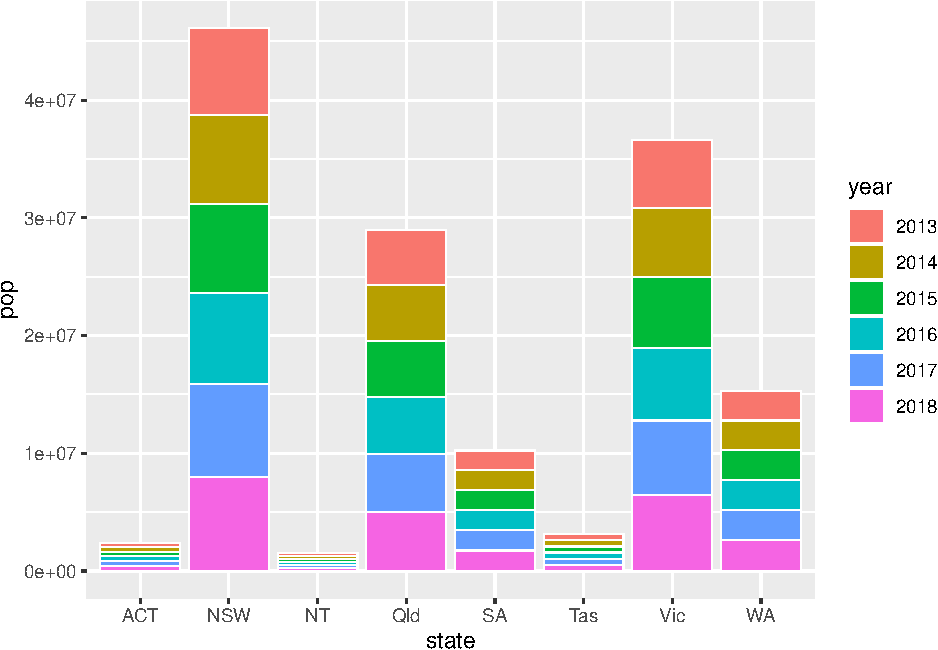
\includegraphics{Data_visualisation_files/figure-latex/complete plot-1.pdf}

Great! Although stacking populations is a bit silly. You can adjust the way \texttt{geoms} work with arguments. In this case, tell it to place the different categories next to each other rather than ontop of each other using \texttt{position\ =\ "dodge"}:

\begin{Shaded}
\begin{Highlighting}[]
\NormalTok{population_table }\OperatorTok\StringTok{ }
\StringTok{        }\KeywordTok{ggplot}\NormalTok{(}\KeywordTok{aes}\NormalTok{(}\DataTypeTok{x =}\NormalTok{ state,}
                   \DataTypeTok{y =}\NormalTok{ pop,}
                   \DataTypeTok{fill =}\NormalTok{ year)) }\OperatorTok{+}
\StringTok{        }\KeywordTok{geom_col}\NormalTok{(}\DataTypeTok{position =} \StringTok{"dodge"}\NormalTok{)}
\end{Highlighting}
\end{Shaded}

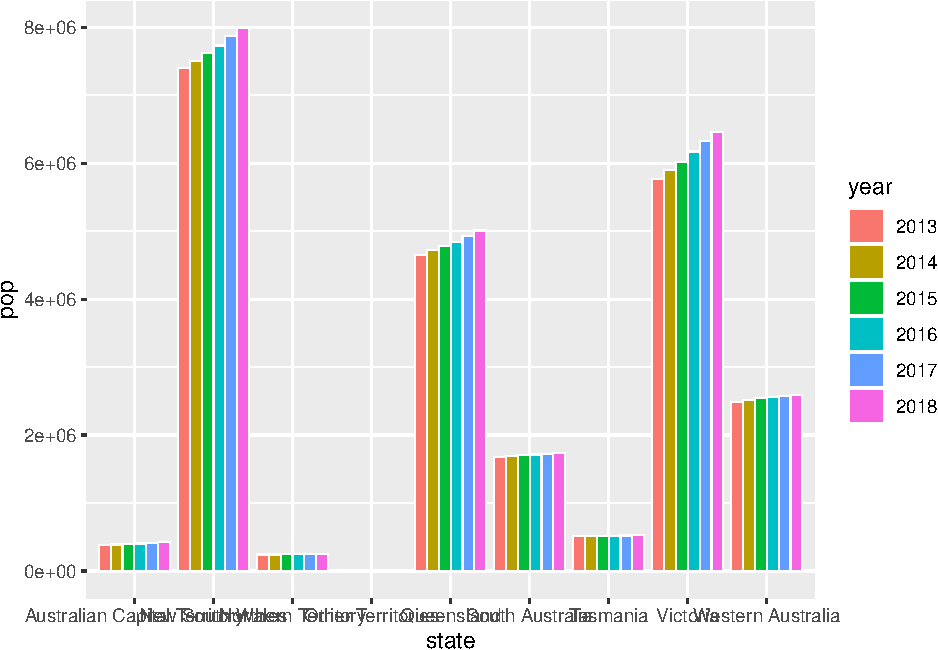
\includegraphics{Data_visualisation_files/figure-latex/with dodge-1.pdf}

That's nicer. The following sections in this chapter will build on this chart. The rest of the chapter will explore:

\begin{itemize}
\tightlist
\item
  Grattanising your charts and choosing colours
\item
  Saving charts according to Grattan templates
\item
  Making bar, line, scatter and distribution plots
\item
  Making maps and interactive charts
\item
  Adding chart labels
\end{itemize}

\hypertarget{making-grattan-y-charts}{%
\section{Making Grattan-y charts}\label{making-grattan-y-charts}}

The \texttt{grattantheme} package contains functions that help \emph{Grattanise} your charts. It is hosted here: \url{https://github.com/mattcowgill/grattantheme}

You can install it with \texttt{devtools::install\_github} from the package:

\begin{Shaded}
\begin{Highlighting}[]
\KeywordTok{install.packages}\NormalTok{(}\StringTok{"devtools"}\NormalTok{)}
\NormalTok{remotes}\OperatorTok{::}\KeywordTok{install_github}\NormalTok{(}\StringTok{"mattcowgill/grattantheme"}\NormalTok{)}
\end{Highlighting}
\end{Shaded}

The key functions of \texttt{grattantheme} are:

\begin{itemize}
\tightlist
\item
  \texttt{theme\_grattan}: set size, font and colour defaults that adhere to the Grattan style guide.
\item
  \texttt{grattan\_y\_continuous}: sets the right defaults for a continuous y-axis.
\item
  \texttt{grattan\_colour\_continuous}: pulls colours from the Grattan colour palete for \texttt{colour} aesthetics.
\item
  \texttt{grattan\_fill\_continuous}: pulls colours from the Grattan colour palete for \texttt{fill} aesthetics.
\item
  \texttt{grattan\_save}: a save function that exports charts in correct report or presentation dimensions.
\end{itemize}

This section will run through some examples of \emph{Grattanising} charts. The \texttt{ggplot} functions are explored in more detail in the next section.

\hypertarget{making-grattan-charts}{%
\subsection{Making Grattan charts}\label{making-grattan-charts}}

Start with a column chart, similar to the one made above:

\begin{Shaded}
\begin{Highlighting}[]
\NormalTok{base_chart <-}\StringTok{ }\NormalTok{population_table }\OperatorTok\StringTok{ }
\StringTok{        }\KeywordTok{ggplot}\NormalTok{(}\KeywordTok{aes}\NormalTok{(}\DataTypeTok{x =}\NormalTok{ state,}
                   \DataTypeTok{y =}\NormalTok{ pop,}
                   \DataTypeTok{fill =}\NormalTok{ year)) }\OperatorTok{+}
\StringTok{        }\KeywordTok{geom_col}\NormalTok{(}\DataTypeTok{position =} \StringTok{"dodge"}\NormalTok{) }\OperatorTok{+}
\StringTok{        }\KeywordTok{labs}\NormalTok{(}\DataTypeTok{x =} \StringTok{""}\NormalTok{,}
             \DataTypeTok{title =} \StringTok{"NSW and Victoria are booming"}\NormalTok{,}
             \DataTypeTok{subtitle =} \StringTok{"Population by state, 2013-2018"}\NormalTok{,}
             \DataTypeTok{caption =} \StringTok{"Source: ABS Regional Dataset (2019)"}\NormalTok{)}

\NormalTok{base_chart}
\end{Highlighting}
\end{Shaded}

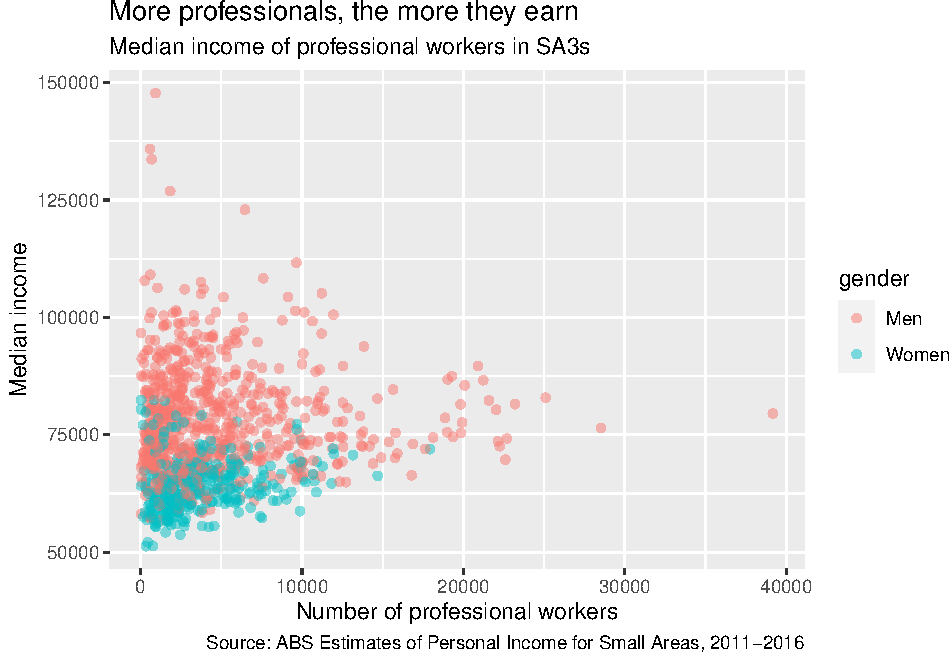
\includegraphics{Data_visualisation_files/figure-latex/base_chart-1.pdf}

Let's make it Grattany. First, add \texttt{theme\_grattan} to your plot:

\begin{Shaded}
\begin{Highlighting}[]
\NormalTok{base_chart }\OperatorTok{+}
\StringTok{        }\KeywordTok{theme_grattan}\NormalTok{()}
\end{Highlighting}
\end{Shaded}

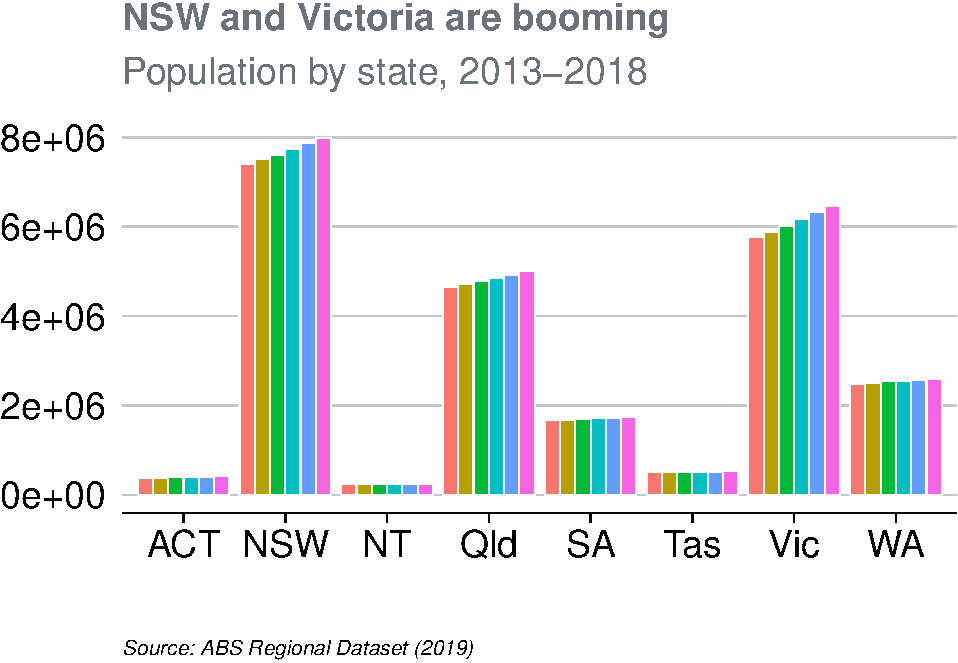
\includegraphics{Data_visualisation_files/figure-latex/add_theme_grattan-1.pdf}

Then \texttt{grattan\_y\_continuous} to align the x-axis with zero. This function takes the same arguments as \texttt{scale\_y\_continuous}, so you can add \texttt{labels\ =\ comma()} to reformat the y-axis labels:

\begin{Shaded}
\begin{Highlighting}[]
\NormalTok{base_chart }\OperatorTok{+}
\StringTok{        }\KeywordTok{theme_grattan}\NormalTok{() }\OperatorTok{+}
\StringTok{        }\KeywordTok{grattan_y_continuous}\NormalTok{(}\DataTypeTok{labels =}\NormalTok{ comma)}
\end{Highlighting}
\end{Shaded}

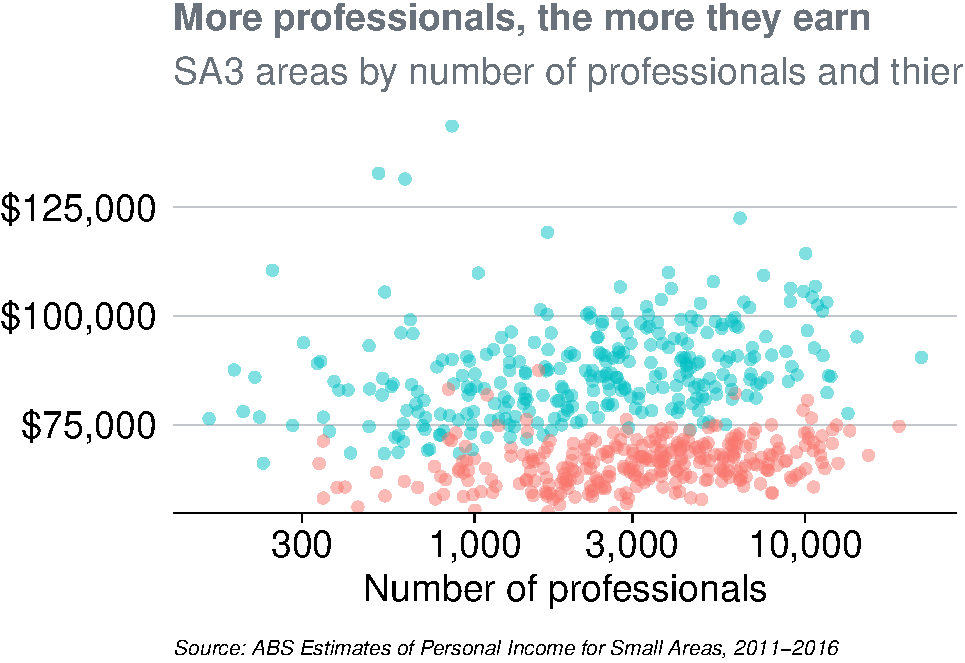
\includegraphics{Data_visualisation_files/figure-latex/add_grattan_y_continuous-1.pdf}

To define \texttt{fill} colours, use \texttt{grattan\_fill\_manual} with the number of colours you need (six, in this case):

\begin{Shaded}
\begin{Highlighting}[]
\NormalTok{pop_chart <-}\StringTok{ }\NormalTok{base_chart }\OperatorTok{+}
\StringTok{        }\KeywordTok{theme_grattan}\NormalTok{() }\OperatorTok{+}
\StringTok{        }\KeywordTok{grattan_y_continuous}\NormalTok{(}\DataTypeTok{labels =}\NormalTok{ comma) }\OperatorTok{+}
\StringTok{        }\KeywordTok{grattan_fill_manual}\NormalTok{(}\DecValTok{6}\NormalTok{)}

\NormalTok{pop_chart}
\end{Highlighting}
\end{Shaded}

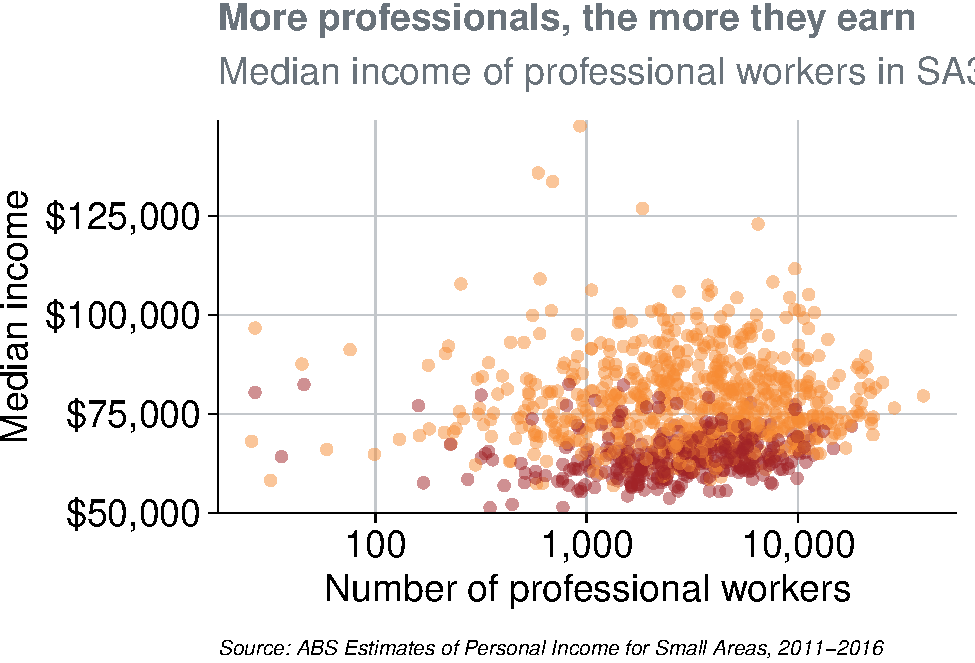
\includegraphics{Data_visualisation_files/figure-latex/add_fill-1.pdf}

Nice chart! Now you can save it and share it with the world.

\hypertarget{saving-grattan-charts}{%
\subsection{Saving Grattan charts}\label{saving-grattan-charts}}

The \texttt{grattan\_save} function saves your charts according to Grattan templates. It takes these arguments:

\begin{itemize}
\tightlist
\item
  \texttt{filename}: the path, name and file-type of your saved chart. eg: \texttt{"atlas/population\_chart.pdf"}.
\item
  \texttt{object}: the R object that you want to save. eg: \texttt{pop\_chart}. If left blank, it grabs the last chart that was displayed.
\item
  \texttt{type}: the Grattan template to be used. This is one of:

  \begin{itemize}
  \tightlist
  \item
    \texttt{"normal"} The default. Use for normal Grattan report charts, or to paste into a 4:3 Powerpoint slide. Width: 22.2cm, height: 14.5cm.
  \item
    \texttt{"normal\_169"} Only useful for pasting into a 16:9 format Grattan Powerpoint slide. Width: 30cm, height: 14.5cm.
  \item
    \texttt{"tiny"} Fills the width of a column in a Grattan report, but is shorter than usual. Width: 22.2cm, height: 11.1cm.
  \item
    \texttt{"wholecolumn"} Takes up a whole column in a Grattan report. Width: 22.2cm, height: 22.2cm.
  \item
    \texttt{"fullpage"} Fills a whole page of a Grattan report. Width: 44.3cm, height: 22.2cm.
  \item
    \texttt{"fullslide"} Creates an image that looks like a 4:3 Grattan Powerpoint slide, complete with logo. Width: 25.4cm, height: 19.0cm.
  \item
    \texttt{"fullslide\_169"} Creates` an image that looks like a 16:9 Grattan Powerpoint slide, complete with logo. Use this to drop into standard presentations. Width: 33.9cm, height: 19.0cm
  \item
    \texttt{"blog"} Creates a 4:3 image that looks like a Grattan Powerpoint slide, but with less border whitespace than `fullslide'."
  \item
    \texttt{"fullslide\_44"\ Creates} an image that looks like a 4:4 Grattan Powerpoint slide. This may be useful for taller charts for the Grattan blog; not useful for any other purpose. Width: 25.4cm, height: 25.4cm.
  \item
    Set \texttt{type\ =\ "all"} to save your chart in all available sizes.
  \end{itemize}
\item
  \texttt{height}: override the height set by \texttt{type}. This can be useful for really long charts in blogposts.
\item
  \texttt{save\_data}: exports a \texttt{csv} file containing the data used in the chart.
\item
  \texttt{force\_labs}: override the removal of labels for a particular \texttt{type}. eg \texttt{force\_labs\ =\ TRUE} will keep the y-axis label.
\end{itemize}

To save the \texttt{pop\_chart} plot created above as a whole-column chart for a \textbf{report}:

\begin{Shaded}
\begin{Highlighting}[]
\KeywordTok{grattan_save}\NormalTok{(}\StringTok{"atlas/population_chart_report.pdf"}\NormalTok{, pop_chart, }\DataTypeTok{type =} \StringTok{"wholecolumn"}\NormalTok{)}
\end{Highlighting}
\end{Shaded}

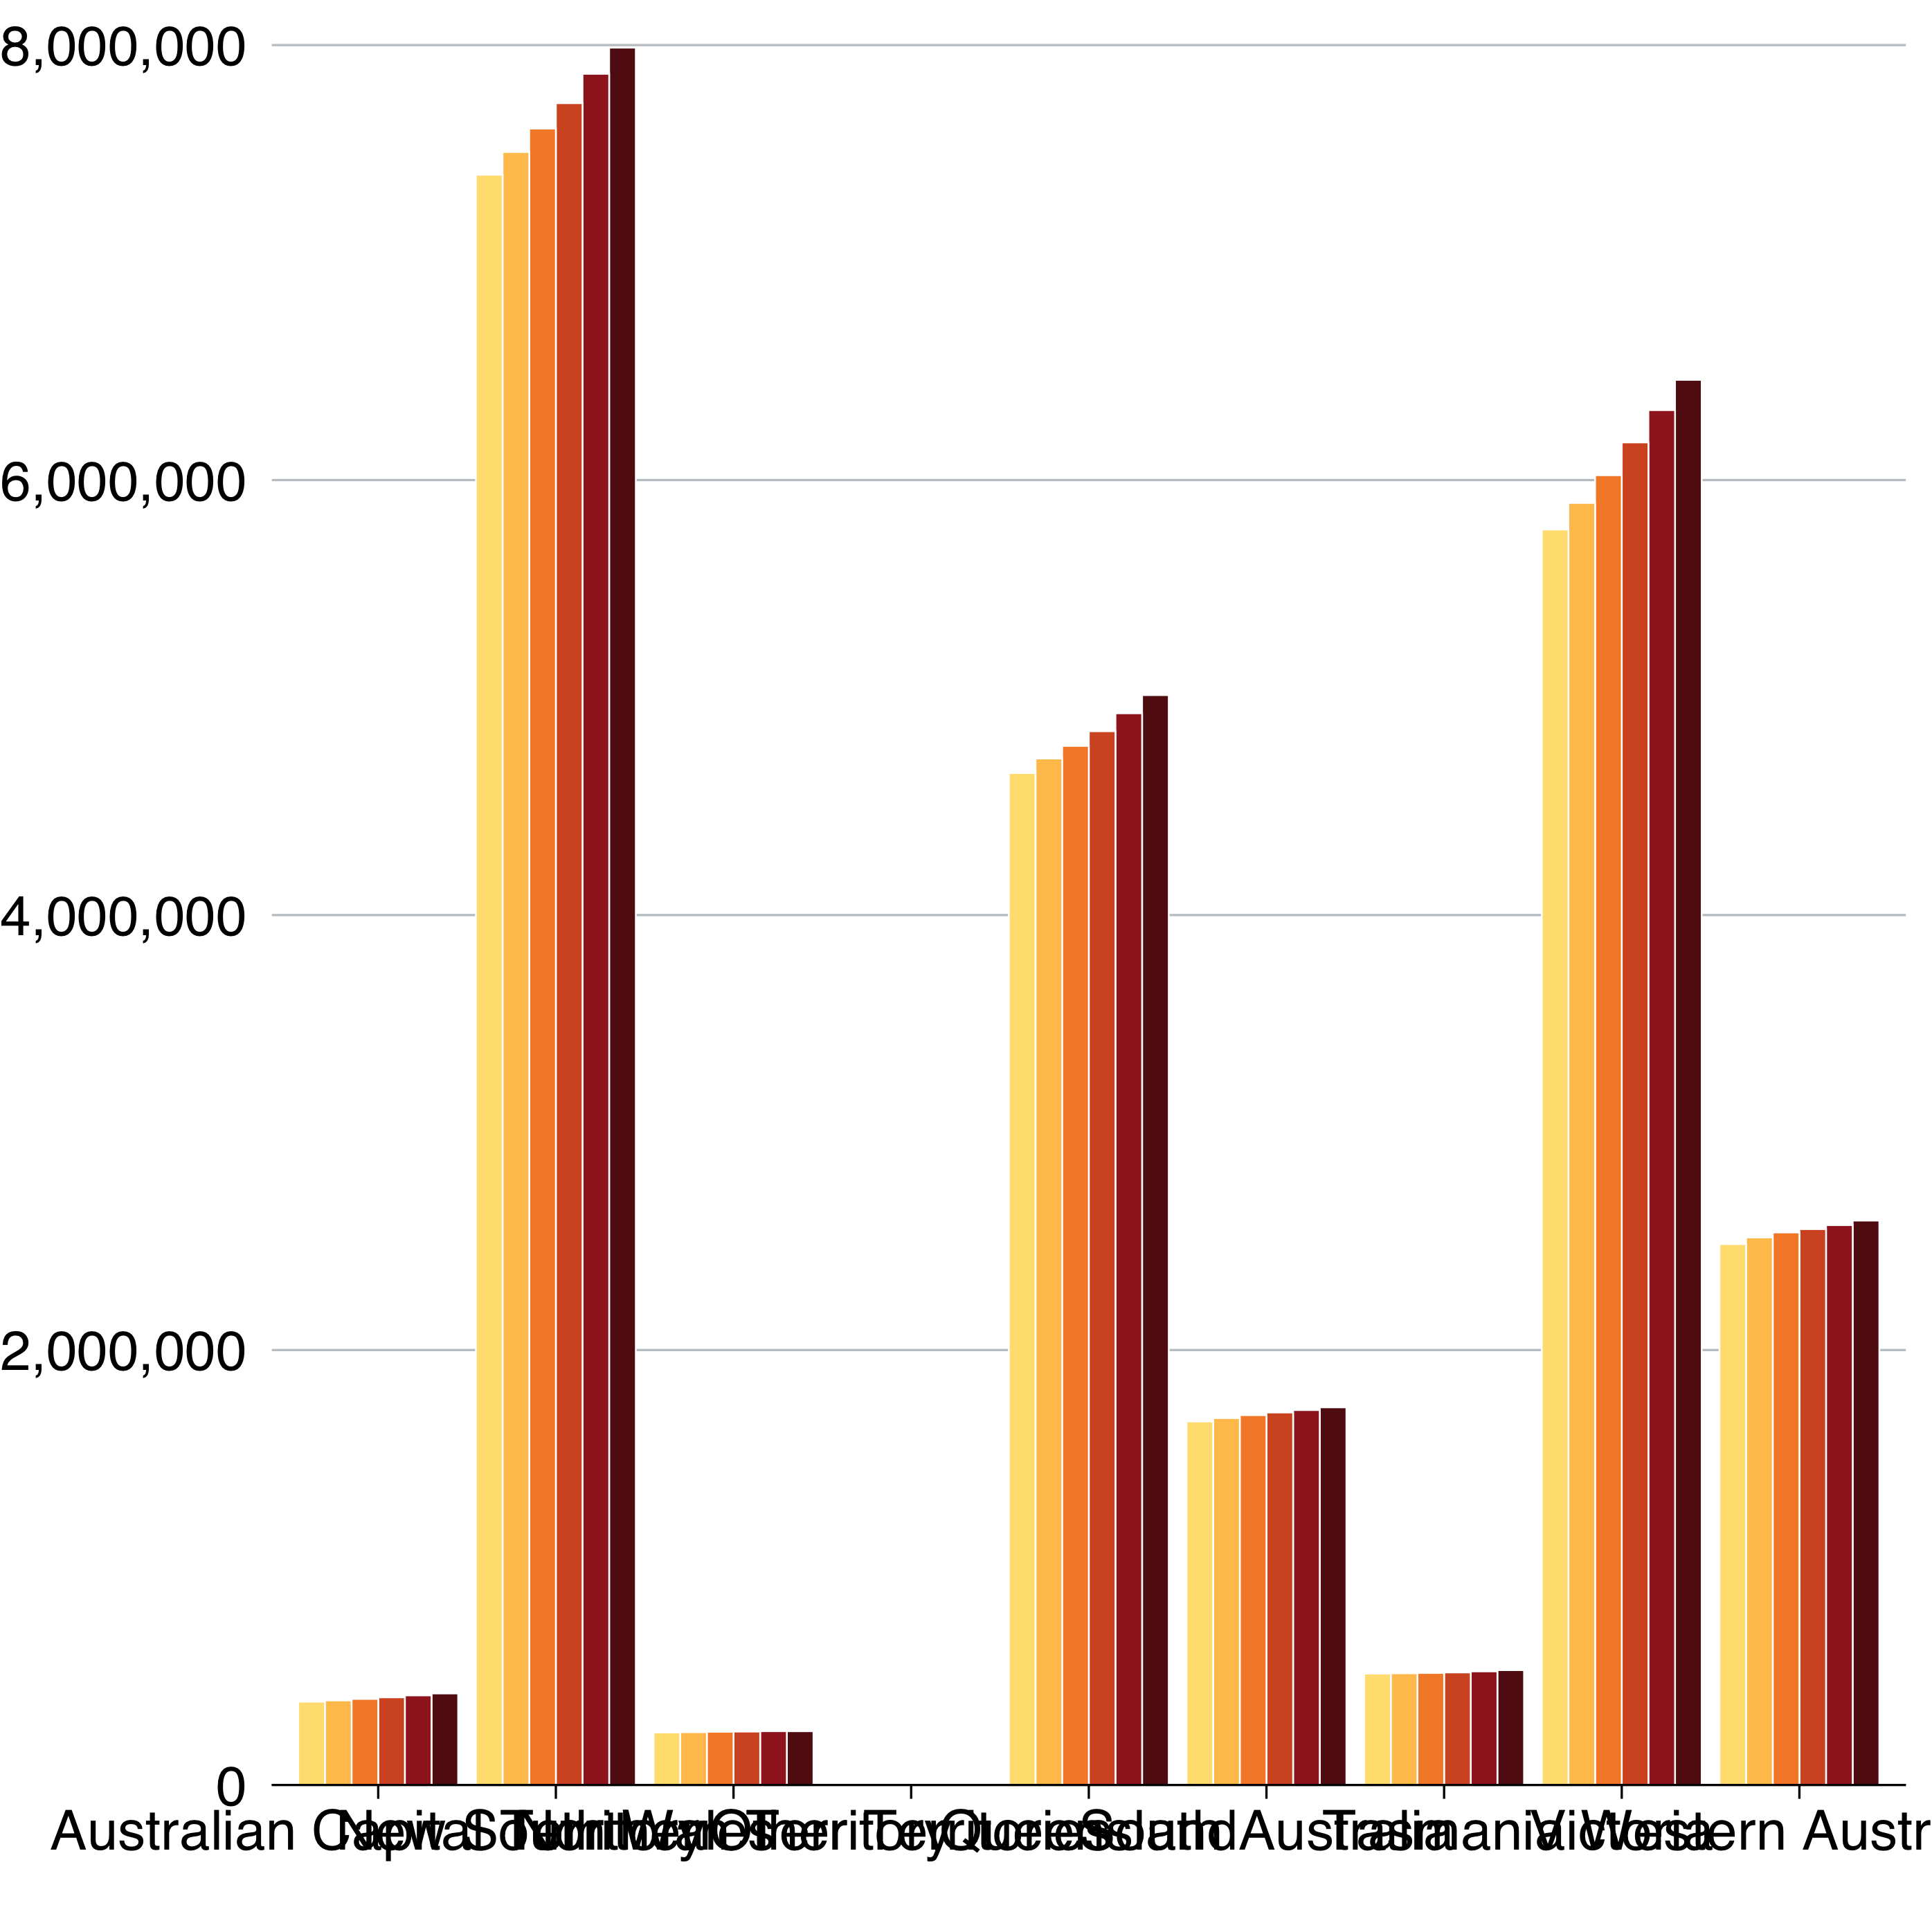
\includegraphics[width=38.76in]{atlas/population_chart_report}

To save it as a \textbf{presentation} slide instead, use \texttt{type\ =\ "fullslide"}:

\begin{Shaded}
\begin{Highlighting}[]
\KeywordTok{grattan_save}\NormalTok{(}\StringTok{"atlas/population_chart_presentation.pdf"}\NormalTok{, pop_chart, }\DataTypeTok{type =} \StringTok{"fullslide"}\NormalTok{)}
\end{Highlighting}
\end{Shaded}

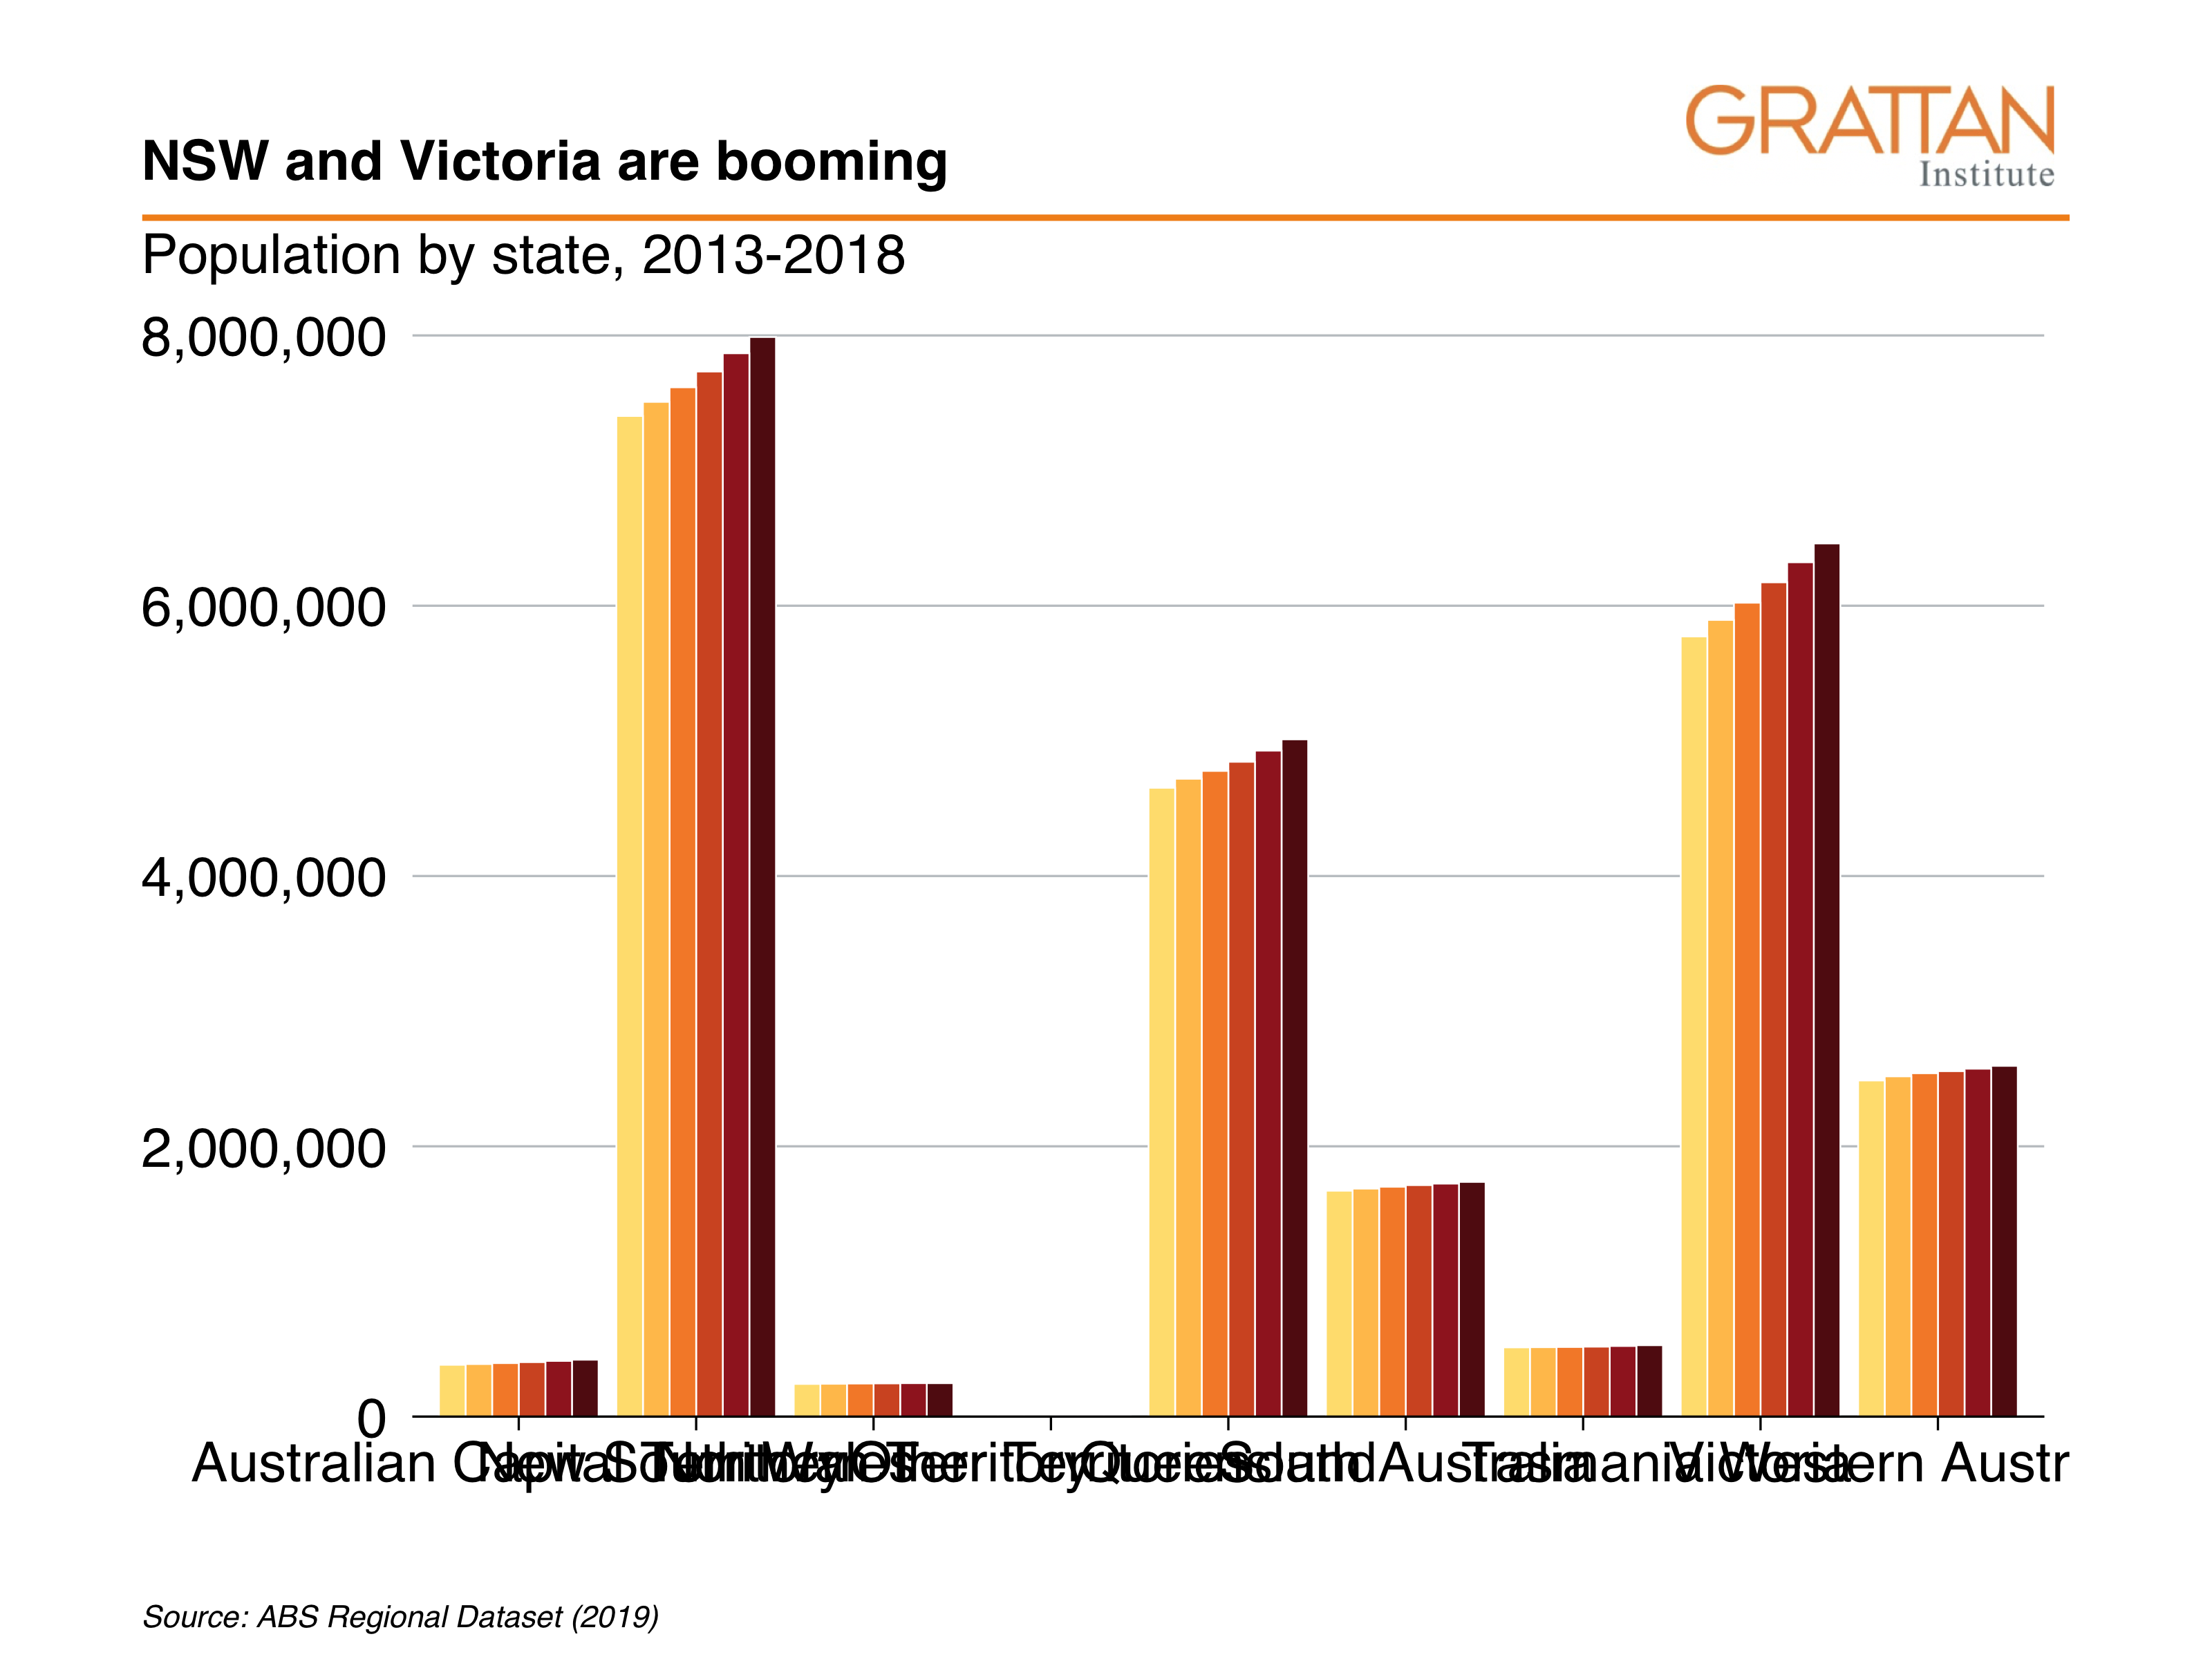
\includegraphics[width=44.44in]{atlas/population_chart_presentation}

Or, if you want to emphasise the point in a \emph{really tall} chart for a \textbf{blogpost}, you can use \texttt{type\ =\ "blog"} and adjust the \texttt{height} to be 50cm. Also note that because this is for the blog, you should save it as a \texttt{png} file:

\begin{Shaded}
\begin{Highlighting}[]
\KeywordTok{grattan_save}\NormalTok{(}\StringTok{"atlas/population_chart_blog.png"}\NormalTok{, pop_chart, }
             \DataTypeTok{type =} \StringTok{"blog"}\NormalTok{, }\DataTypeTok{height =} \DecValTok{50}\NormalTok{)}
\end{Highlighting}
\end{Shaded}

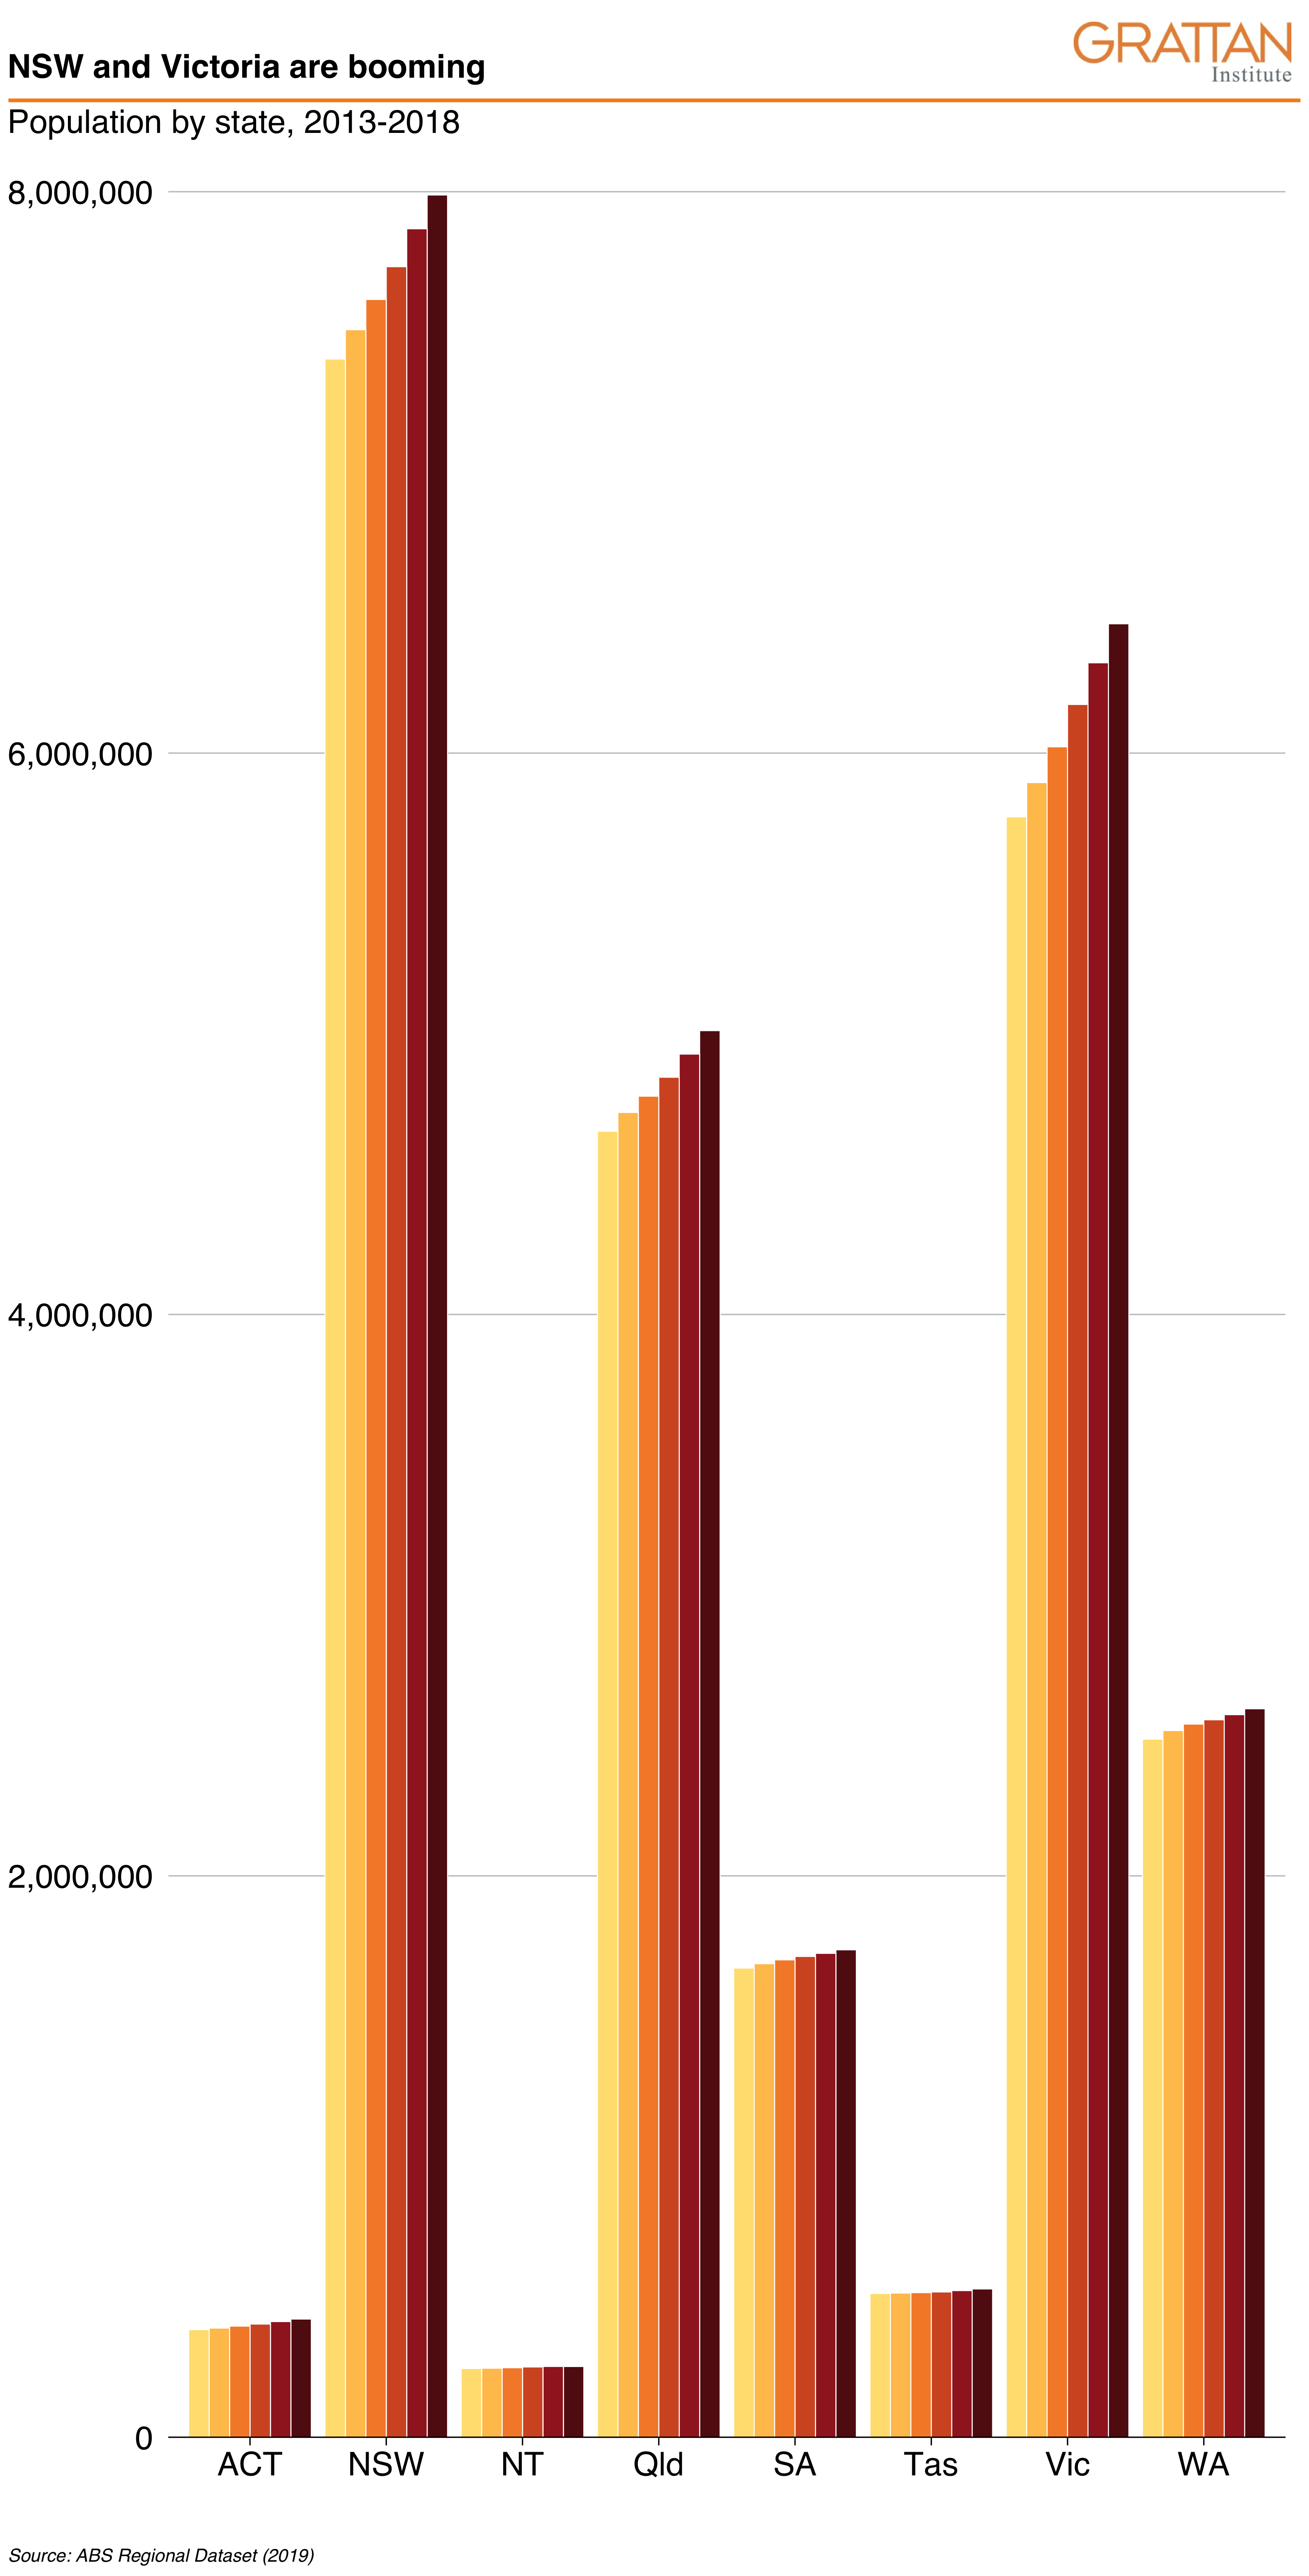
\includegraphics[width=44.44in]{atlas/population_chart_blog}

And that's it! The following sections will go into more detail about different chart types in R, but you'll mostly use the same basic \texttt{grattantheme} formatting you've used here.

\hypertarget{chart-cookbook}{%
\section{Chart cookbook}\label{chart-cookbook}}

This section takes you through a few often-used chart types.

\hypertarget{bar-charts}{%
\subsection{Bar charts}\label{bar-charts}}

Bar charts are made with \texttt{geom\_bar} or \texttt{geom\_col}. Creating a bar chart will look something like this:

\begin{Shaded}
\begin{Highlighting}[]
\KeywordTok{ggplot}\NormalTok{(}\DataTypeTok{data =} \OperatorTok{<}\NormalTok{data}\OperatorTok{>}\NormalTok{) }\OperatorTok{+}\StringTok{ }
\StringTok{  }\KeywordTok{geom_bar}\NormalTok{(}\KeywordTok{aes}\NormalTok{(}\DataTypeTok{x =} \OperatorTok{<}\NormalTok{xvar}\OperatorTok{>}\NormalTok{, }\DataTypeTok{y =} \OperatorTok{<}\NormalTok{yvar}\OperatorTok{>}\NormalTok{),}
     \DataTypeTok{stat =} \OperatorTok{<}\NormalTok{STAT}\OperatorTok{>}\NormalTok{, }
     \DataTypeTok{position =} \OperatorTok{<}\NormalTok{POSITION}\OperatorTok{>}
\StringTok{  }\NormalTok{)}
\end{Highlighting}
\end{Shaded}

It has two key arguments: \texttt{stat} and \texttt{position}.

First, \texttt{stat} defines what kind of \emph{operation} the function will do on the dataset before plotting. Some options are:

\begin{itemize}
\tightlist
\item
  \texttt{"count"}, the default: count the number of observations in a particular group, and plot that number. This is useful when you're using microdata. When this is the case, there is no need for a \texttt{y} aesthetic.
\item
  \texttt{"sum"}: sum the values of the \texttt{y} aesthetic.
\item
  \texttt{"identity"}: directly report the values of the \texttt{y} aesthetic. This is how Powerpoint and Excel charts work.
\end{itemize}

You can use \texttt{geom\_col} instead, as a shortcut for \texttt{geom\_bar(stat\ =\ "identity)}.

Second, \texttt{position}, dictates how multiple bars occupying the same x-axis position will positioned. The options are:

\begin{itemize}
\tightlist
\item
  \texttt{"stack"}, the default: bars in the same group are stacked atop one another.
\item
  \texttt{"dodge"}: bars in the same group are positioned next to one another.
\item
  \texttt{"fill"}: bars in the same group are stacked and all fill to 100 per cent.
\end{itemize}

\begin{Shaded}
\begin{Highlighting}[]
\NormalTok{population_table }\OperatorTok\StringTok{ }
\StringTok{        }\KeywordTok{ggplot}\NormalTok{(}\KeywordTok{aes}\NormalTok{(}\DataTypeTok{x =}\NormalTok{ state,}
                   \DataTypeTok{y =}\NormalTok{ pop,}
                   \DataTypeTok{fill =}\NormalTok{ year)) }\OperatorTok{+}
\StringTok{        }\KeywordTok{geom_bar}\NormalTok{(}\DataTypeTok{stat =} \StringTok{"identity"}\NormalTok{,}
                 \DataTypeTok{position =} \StringTok{"dodge"}\NormalTok{) }\OperatorTok{+}
\StringTok{        }\KeywordTok{theme_grattan}\NormalTok{() }\OperatorTok{+}
\StringTok{        }\KeywordTok{grattan_y_continuous}\NormalTok{(}\DataTypeTok{labels =}\NormalTok{ comma) }\OperatorTok{+}
\StringTok{        }\KeywordTok{grattan_fill_manual}\NormalTok{(}\DecValTok{6}\NormalTok{)}
\end{Highlighting}
\end{Shaded}

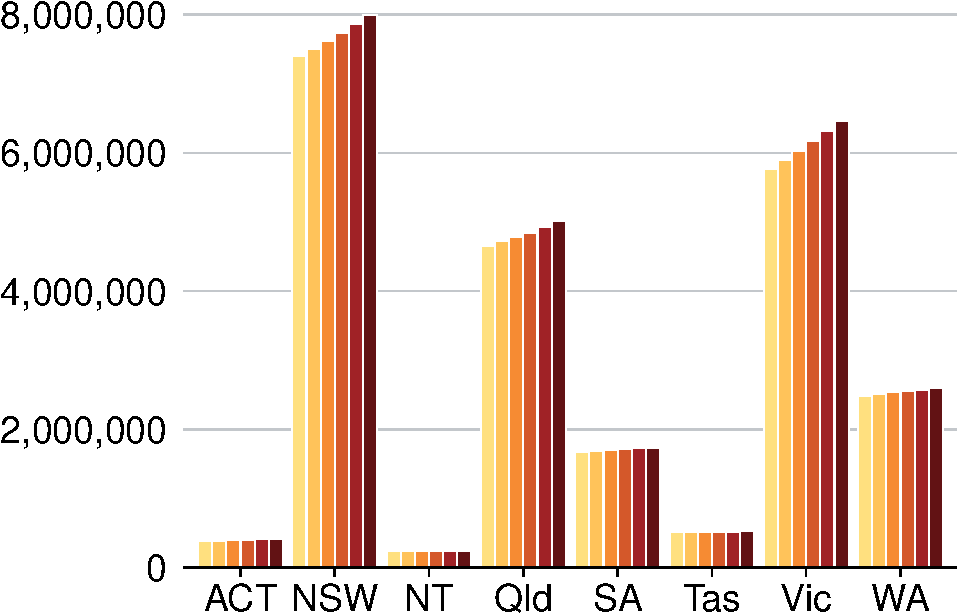
\includegraphics{Data_visualisation_files/figure-latex/bar2-1.pdf}

You can also \textbf{order} the groups in your chart by a variable. If you want to order states by population, use \texttt{reorder} inside \texttt{aes}:

\begin{Shaded}
\begin{Highlighting}[]
\NormalTok{population_table }\OperatorTok\StringTok{ }
\StringTok{        }\KeywordTok{ggplot}\NormalTok{(}\KeywordTok{aes}\NormalTok{(}\DataTypeTok{x =} \KeywordTok{reorder}\NormalTok{(state, }\OperatorTok{-}\NormalTok{pop), }\CommentTok{# reorder state by negative population}
                   \DataTypeTok{y =}\NormalTok{ pop,}
                   \DataTypeTok{fill =}\NormalTok{ year)) }\OperatorTok{+}
\StringTok{        }\KeywordTok{geom_bar}\NormalTok{(}\DataTypeTok{stat =} \StringTok{"identity"}\NormalTok{,}
                 \DataTypeTok{position =} \StringTok{"dodge"}\NormalTok{) }\OperatorTok{+}
\StringTok{        }\KeywordTok{theme_grattan}\NormalTok{() }\OperatorTok{+}
\StringTok{        }\KeywordTok{grattan_y_continuous}\NormalTok{(}\DataTypeTok{labels =}\NormalTok{ comma) }\OperatorTok{+}
\StringTok{        }\KeywordTok{grattan_fill_manual}\NormalTok{(}\DecValTok{6}\NormalTok{) }\OperatorTok{+}\StringTok{ }
\StringTok{        }\KeywordTok{labs}\NormalTok{(}\DataTypeTok{x =} \StringTok{""}\NormalTok{)}
\end{Highlighting}
\end{Shaded}

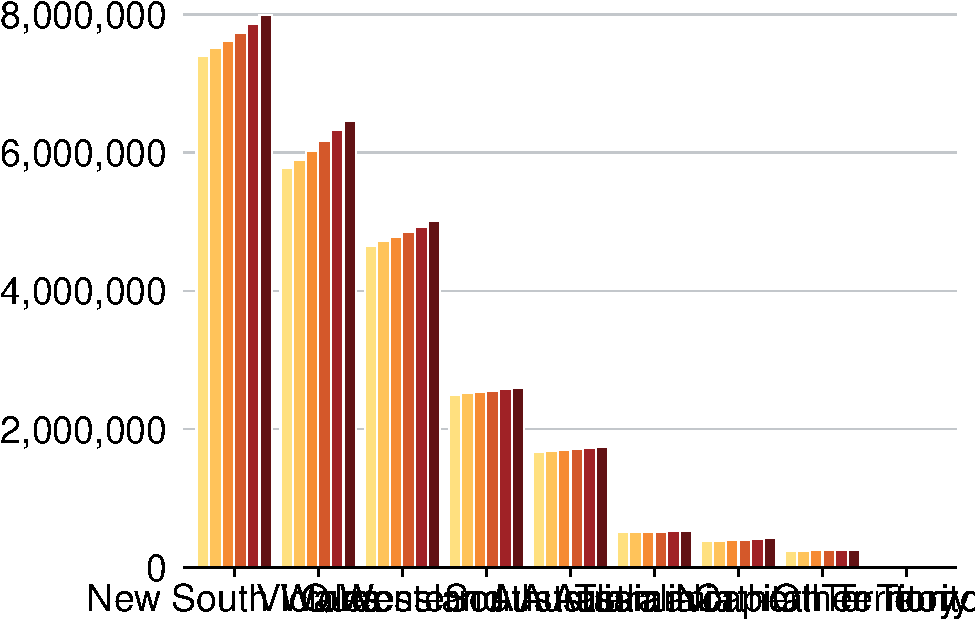
\includegraphics{Data_visualisation_files/figure-latex/bar3-1.pdf}

To flip the chart -- a useful move when you have long labels -- add \texttt{coord\_flipped} (ie `flip coordinates') and tell \texttt{theme\_grattan} that the plot is flipped using \texttt{flipped\ =\ TRUE}.

\begin{Shaded}
\begin{Highlighting}[]
\NormalTok{population_table }\OperatorTok\StringTok{ }
\StringTok{        }\KeywordTok{ggplot}\NormalTok{(}\KeywordTok{aes}\NormalTok{(}\DataTypeTok{x =} \KeywordTok{reorder}\NormalTok{(state, }\OperatorTok{-}\NormalTok{pop), }
                   \DataTypeTok{y =}\NormalTok{ pop,}
                   \DataTypeTok{fill =}\NormalTok{ year)) }\OperatorTok{+}
\StringTok{        }\KeywordTok{geom_bar}\NormalTok{(}\DataTypeTok{stat =} \StringTok{"identity"}\NormalTok{,}
                 \DataTypeTok{position =} \StringTok{"dodge"}\NormalTok{) }\OperatorTok{+}
\StringTok{        }\KeywordTok{coord_flip}\NormalTok{() }\OperatorTok{+}\StringTok{  }\CommentTok{# flip the coordinates}
\StringTok{        }\KeywordTok{theme_grattan}\NormalTok{(}\DataTypeTok{flipped =} \OtherTok{TRUE}\NormalTok{) }\OperatorTok{+}\StringTok{  }\CommentTok{# tell theme_grattan}
\StringTok{        }\KeywordTok{grattan_y_continuous}\NormalTok{(}\DataTypeTok{labels =}\NormalTok{ comma) }\OperatorTok{+}
\StringTok{        }\KeywordTok{grattan_fill_manual}\NormalTok{(}\DecValTok{6}\NormalTok{) }\OperatorTok{+}\StringTok{ }
\StringTok{        }\KeywordTok{labs}\NormalTok{(}\DataTypeTok{x =} \StringTok{""}\NormalTok{)}
\end{Highlighting}
\end{Shaded}

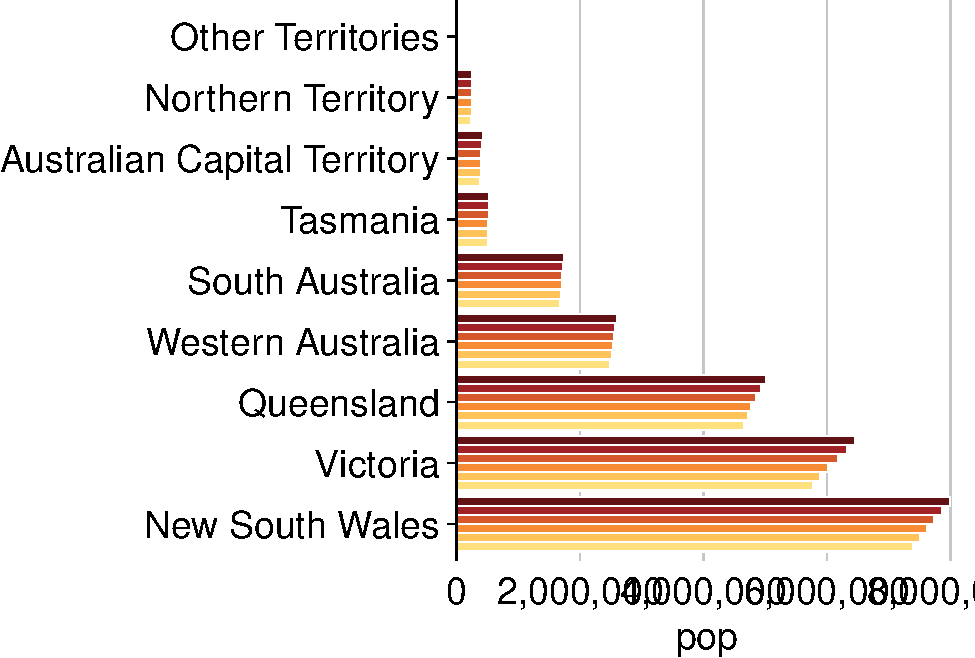
\includegraphics{Data_visualisation_files/figure-latex/bar4-1.pdf}

\hypertarget{line-charts}{%
\subsection{Line charts}\label{line-charts}}

A line chart has one key aesthetic: \texttt{group}. This tells \texttt{ggplot} how to connect individual lines.

\begin{Shaded}
\begin{Highlighting}[]
\NormalTok{population_table }\OperatorTok\StringTok{ }
\StringTok{        }\KeywordTok{ggplot}\NormalTok{(}\KeywordTok{aes}\NormalTok{(}\DataTypeTok{x =}\NormalTok{ year,}
                   \DataTypeTok{y =}\NormalTok{ pop,}
                   \DataTypeTok{colour =}\NormalTok{ state,}
                   \DataTypeTok{group =}\NormalTok{ state)) }\OperatorTok{+}
\StringTok{        }\KeywordTok{geom_line}\NormalTok{() }\OperatorTok{+}
\StringTok{        }\KeywordTok{theme_grattan}\NormalTok{() }\OperatorTok{+}
\StringTok{        }\KeywordTok{grattan_y_continuous}\NormalTok{(}\DataTypeTok{labels =}\NormalTok{ comma) }\OperatorTok{+}
\StringTok{        }\KeywordTok{grattan_colour_manual}\NormalTok{(}\DecValTok{9}\NormalTok{) }\OperatorTok{+}
\StringTok{        }\KeywordTok{labs}\NormalTok{(}\DataTypeTok{x =} \StringTok{""}\NormalTok{)}
\end{Highlighting}
\end{Shaded}

\begin{verbatim}
## Warning in grattantheme::grattan_pal(n = n, reverse = reverse, faded =
## faded): Using more than six colours is not recommended.
\end{verbatim}

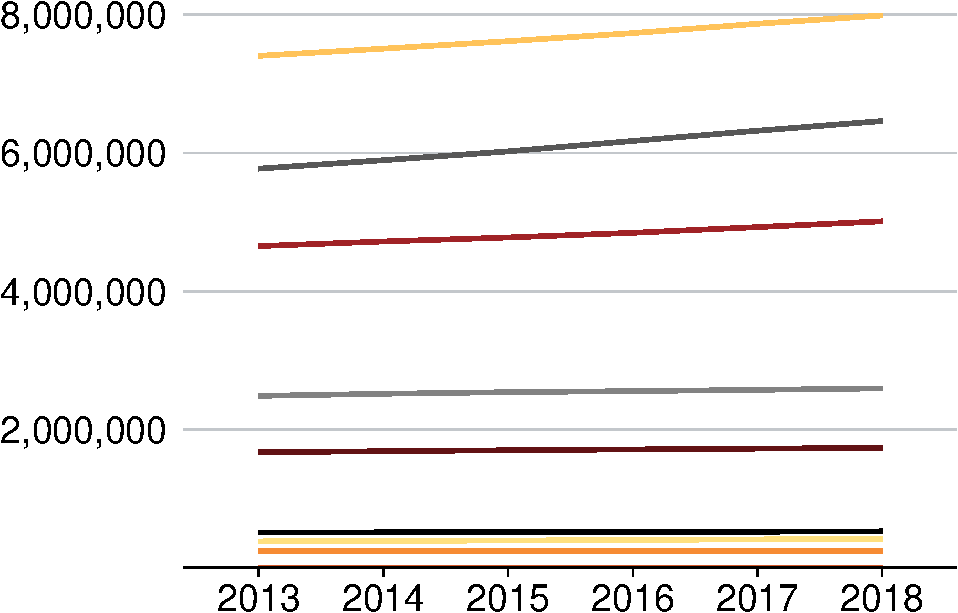
\includegraphics{Data_visualisation_files/figure-latex/line1-1.pdf}

You can also add dots for each year by layering \texttt{geom\_point} on top of \texttt{geom\_line}:

\begin{Shaded}
\begin{Highlighting}[]
\NormalTok{population_table }\OperatorTok\StringTok{ }
\StringTok{        }\KeywordTok{ggplot}\NormalTok{(}\KeywordTok{aes}\NormalTok{(}\DataTypeTok{x =}\NormalTok{ year,}
                   \DataTypeTok{y =}\NormalTok{ pop,}
                   \DataTypeTok{colour =}\NormalTok{ state,}
                   \DataTypeTok{group =}\NormalTok{ state)) }\OperatorTok{+}
\StringTok{        }\KeywordTok{geom_line}\NormalTok{() }\OperatorTok{+}
\StringTok{        }\KeywordTok{geom_point}\NormalTok{(}\DataTypeTok{size =} \DecValTok{2}\NormalTok{) }\OperatorTok{+}\StringTok{ }
\StringTok{        }\KeywordTok{theme_grattan}\NormalTok{() }\OperatorTok{+}
\StringTok{        }\KeywordTok{grattan_y_continuous}\NormalTok{(}\DataTypeTok{labels =}\NormalTok{ comma) }\OperatorTok{+}
\StringTok{        }\KeywordTok{grattan_colour_manual}\NormalTok{(}\DecValTok{9}\NormalTok{) }\OperatorTok{+}\StringTok{ }
\StringTok{        }\KeywordTok{labs}\NormalTok{(}\DataTypeTok{x =} \StringTok{""}\NormalTok{)}
\end{Highlighting}
\end{Shaded}

\begin{verbatim}
## Warning in grattantheme::grattan_pal(n = n, reverse = reverse, faded =
## faded): Using more than six colours is not recommended.
\end{verbatim}

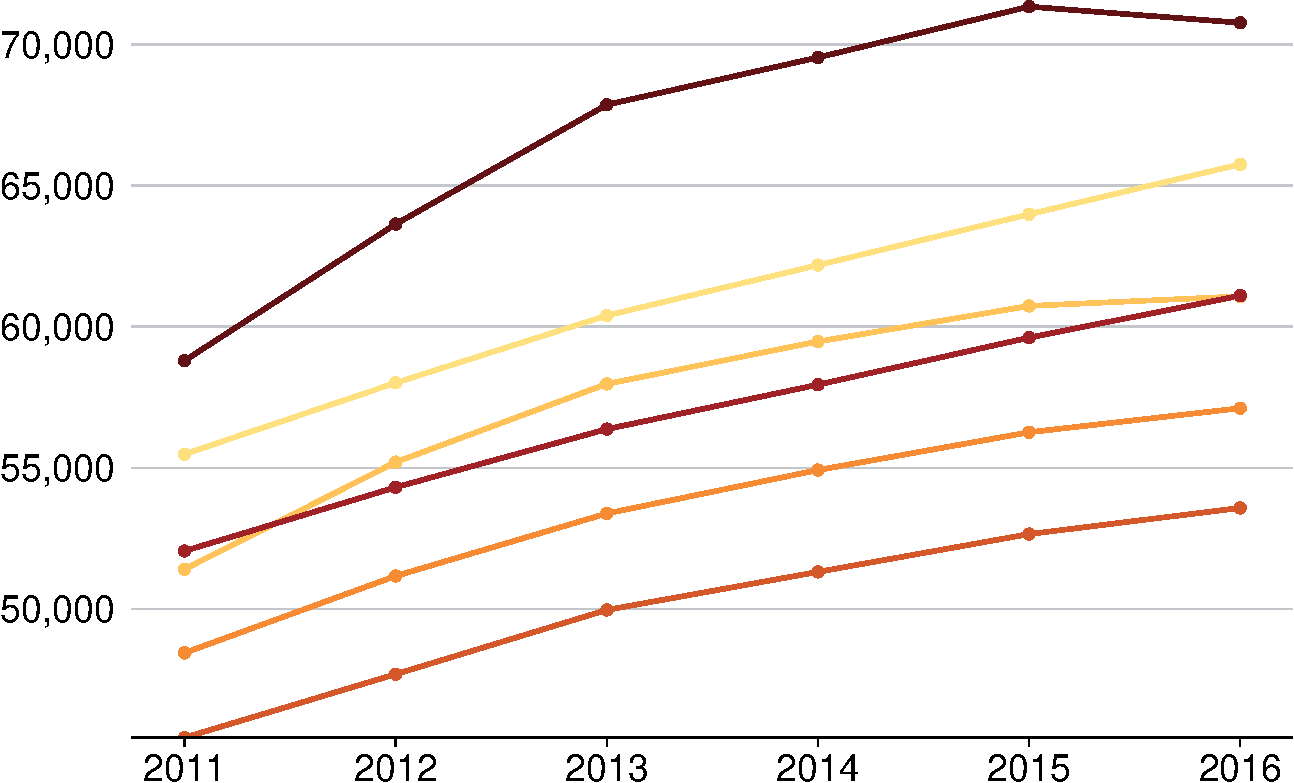
\includegraphics{Data_visualisation_files/figure-latex/line2-1.pdf}

If you wanted to show each state individually, you could \textbf{facet} your chart so that a separate plot was produced for each state:

\begin{Shaded}
\begin{Highlighting}[]
\NormalTok{population_table }\OperatorTok\StringTok{ }
\StringTok{        }\KeywordTok{filter}\NormalTok{(state }\OperatorTok{!=}\StringTok{ "ACT"}\NormalTok{,}
\NormalTok{               state }\OperatorTok{!=}\StringTok{ "NT"}\NormalTok{) }\OperatorTok\StringTok{ }
\StringTok{        }\KeywordTok{ggplot}\NormalTok{(}\KeywordTok{aes}\NormalTok{(}\DataTypeTok{x =}\NormalTok{ year,}
                   \DataTypeTok{y =}\NormalTok{ pop,}
                   \DataTypeTok{group =}\NormalTok{ state)) }\OperatorTok{+}
\StringTok{        }\KeywordTok{geom_line}\NormalTok{() }\OperatorTok{+}
\StringTok{        }\KeywordTok{geom_point}\NormalTok{(}\DataTypeTok{size =} \DecValTok{2}\NormalTok{) }\OperatorTok{+}\StringTok{ }
\StringTok{        }\KeywordTok{theme_grattan}\NormalTok{() }\OperatorTok{+}
\StringTok{        }\KeywordTok{grattan_y_continuous}\NormalTok{() }\OperatorTok{+}
\StringTok{        }\KeywordTok{facet_wrap}\NormalTok{(state }\OperatorTok{~}\StringTok{ }\NormalTok{.) }\OperatorTok{+}\StringTok{ }
\StringTok{        }\KeywordTok{labs}\NormalTok{(}\DataTypeTok{x =} \StringTok{""}\NormalTok{)}
\end{Highlighting}
\end{Shaded}

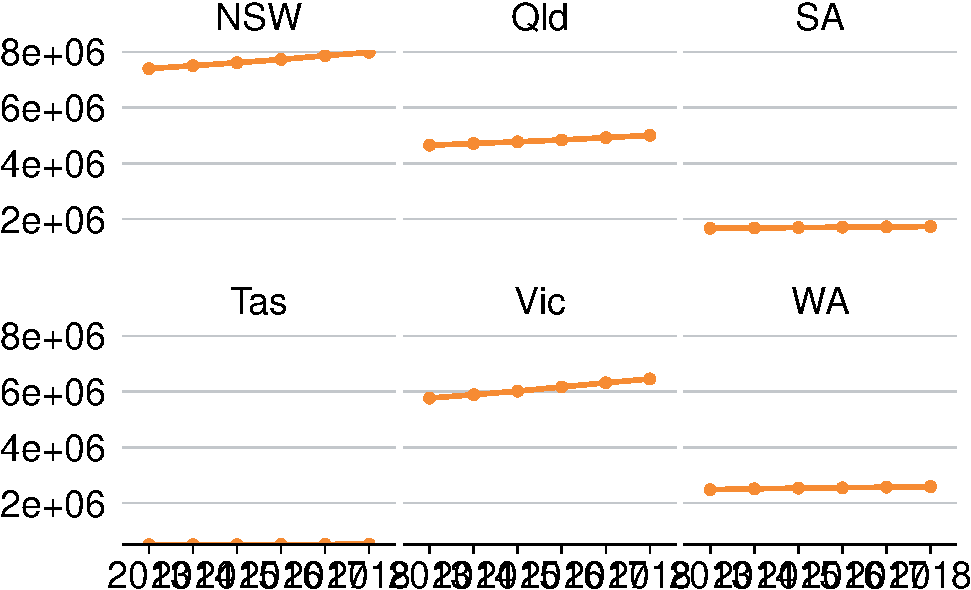
\includegraphics{Data_visualisation_files/figure-latex/line3-1.pdf}

To tidy this up, we can:

\begin{enumerate}
\def\labelenumi{\arabic{enumi}.}
\tightlist
\item
  shorten the years to be ``13'', ``14'', etc instead of ``2013'', ``2014'', etc (via the \texttt{x} aesthetic)
\item
  shorten the y-axis labels to ``millions'' (via the \texttt{y} aesthetic)
\item
  add a black horizontal line at the bottom of each facet
\item
  give the facets a bit of room by adjusting \texttt{panel.spacing}
\item
  define our own x-axis label breaks to just show \texttt{13}, \texttt{15} and \texttt{17}
\end{enumerate}

\begin{Shaded}
\begin{Highlighting}[]
\NormalTok{population_table }\OperatorTok\StringTok{ }
\StringTok{        }\KeywordTok{filter}\NormalTok{(state }\OperatorTok{!=}\StringTok{ "ACT"}\NormalTok{,}
\NormalTok{               state }\OperatorTok{!=}\StringTok{ "NT"}\NormalTok{) }\OperatorTok\StringTok{ }
\StringTok{        }\KeywordTok{ggplot}\NormalTok{(}\KeywordTok{aes}\NormalTok{(}\DataTypeTok{x =} \KeywordTok{substr}\NormalTok{(year, }\DecValTok{3}\NormalTok{, }\DecValTok{4}\NormalTok{), }\CommentTok{# 1: just take the last two characters}
                   \DataTypeTok{y =}\NormalTok{ pop }\OperatorTok{/}\StringTok{ }\FloatTok{1e6}\NormalTok{, }\CommentTok{# 2: divide population by one million}
                   \DataTypeTok{group =}\NormalTok{ state)) }\OperatorTok{+}
\StringTok{        }\KeywordTok{geom_line}\NormalTok{() }\OperatorTok{+}
\StringTok{        }\KeywordTok{geom_point}\NormalTok{(}\DataTypeTok{size =} \DecValTok{2}\NormalTok{) }\OperatorTok{+}\StringTok{ }
\StringTok{        }\KeywordTok{geom_hline}\NormalTok{(}\DataTypeTok{yintercept =} \DecValTok{0}\NormalTok{) }\OperatorTok{+}\StringTok{ }\CommentTok{# 3: add horizontal line at the bottom}
\StringTok{        }\KeywordTok{theme_grattan}\NormalTok{() }\OperatorTok{+}
\StringTok{        }\KeywordTok{theme}\NormalTok{(}\DataTypeTok{panel.spacing =} \KeywordTok{unit}\NormalTok{(}\DecValTok{10}\NormalTok{, }\StringTok{"mm"}\NormalTok{)) }\OperatorTok{+}\StringTok{ }\CommentTok{# 4: add panel spacing}
\StringTok{        }\KeywordTok{grattan_y_continuous}\NormalTok{(}\DataTypeTok{labels =}\NormalTok{ comma) }\OperatorTok{+}
\StringTok{        }\KeywordTok{scale_x_discrete}\NormalTok{(}\DataTypeTok{breaks =} \KeywordTok{c}\NormalTok{(}\StringTok{"13"}\NormalTok{, }\StringTok{"15"}\NormalTok{, }\StringTok{"17"}\NormalTok{)) }\OperatorTok{+}\StringTok{ }\CommentTok{# 5: define our own label breaks}
\StringTok{        }\KeywordTok{facet_wrap}\NormalTok{(state }\OperatorTok{~}\StringTok{ }\NormalTok{.) }\OperatorTok{+}\StringTok{ }
\StringTok{        }\KeywordTok{labs}\NormalTok{(}\DataTypeTok{x =} \StringTok{""}\NormalTok{)}
\end{Highlighting}
\end{Shaded}

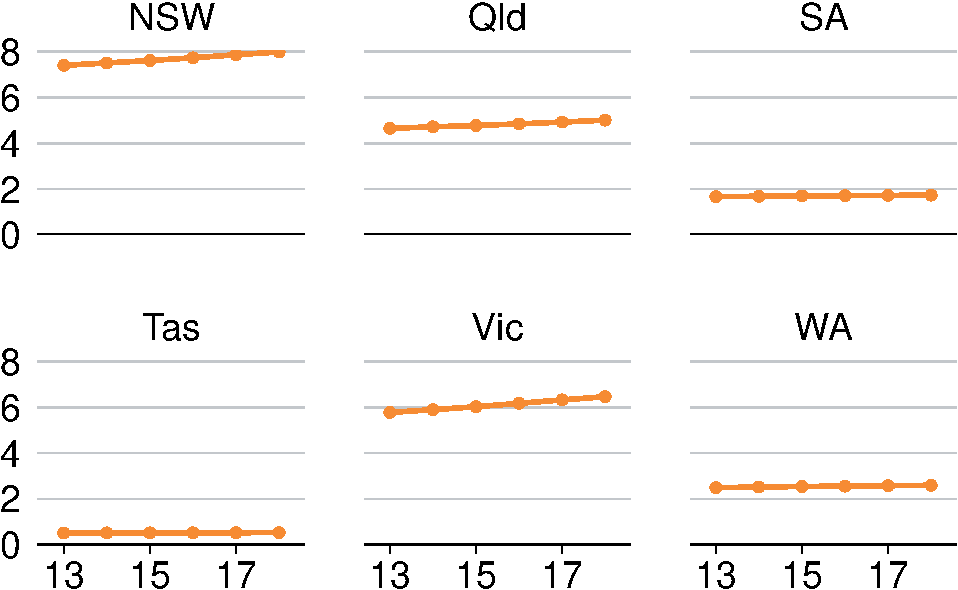
\includegraphics{Data_visualisation_files/figure-latex/line4-1.pdf}

\hypertarget{scatter-plots}{%
\subsection{Scatter plots}\label{scatter-plots}}

Scatter plots require \texttt{x} and \texttt{y} aesthetics. These can then be coloured and facetted.

First, create a dataset that we'll use for scatter plots. Take the \texttt{population\_table} dataset and transform it to have one variable for population in 2013, and another for population in 2018:

\begin{Shaded}
\begin{Highlighting}[]
\NormalTok{population_diff <-}\StringTok{ }\KeywordTok{read_csv}\NormalTok{(}\StringTok{"data/population_sa4.csv"}\NormalTok{) }\OperatorTok\StringTok{ }
\StringTok{        }\KeywordTok{mutate}\NormalTok{(}\DataTypeTok{state_long =}\NormalTok{ state,}
               \DataTypeTok{state =}\NormalTok{ strayr}\OperatorTok{::}\KeywordTok{strayr}\NormalTok{(state_long),}
               \DataTypeTok{pop =} \KeywordTok{as.numeric}\NormalTok{(value),}
               \DataTypeTok{year =} \KeywordTok{as.factor}\NormalTok{(glue}\OperatorTok{::}\KeywordTok{glue}\NormalTok{(}\StringTok{"y\{year\}"}\NormalTok{))) }\OperatorTok\StringTok{ }
\StringTok{        }\KeywordTok{filter}\NormalTok{(year }\OperatorTok\StringTok{ }\KeywordTok{c}\NormalTok{(}\StringTok{"y2013"}\NormalTok{, }\StringTok{"y2018"}\NormalTok{),}
\NormalTok{               data_item }\OperatorTok{==}\StringTok{ "Persons - Total (no.)"}\NormalTok{,}
\NormalTok{               sa4_name }\OperatorTok{!=}\StringTok{ "Other Territories"}\NormalTok{) }\OperatorTok\StringTok{ }
\StringTok{        }\KeywordTok{group_by}\NormalTok{(year, state, sa4_name) }\OperatorTok\StringTok{ }
\StringTok{        }\KeywordTok{summarise}\NormalTok{(}\DataTypeTok{pop =} \KeywordTok{sum}\NormalTok{(pop)) }\OperatorTok\StringTok{ }
\StringTok{        }\KeywordTok{spread}\NormalTok{(year, pop) }\OperatorTok\StringTok{ }
\StringTok{        }\KeywordTok{mutate}\NormalTok{(}\DataTypeTok{pop_change =} \DecValTok{100} \OperatorTok{*}\StringTok{ }\NormalTok{(y2018 }\OperatorTok{/}\StringTok{ }\NormalTok{y2013 }\OperatorTok{-}\StringTok{ }\DecValTok{1}\NormalTok{))}
\end{Highlighting}
\end{Shaded}

\begin{Shaded}
\begin{Highlighting}[]
\NormalTok{population_diff }\OperatorTok\StringTok{ }
\StringTok{        }\KeywordTok{ggplot}\NormalTok{(}\KeywordTok{aes}\NormalTok{(}\DataTypeTok{x =}\NormalTok{ y2013}\OperatorTok{/}\DecValTok{1000}\NormalTok{,}
                   \DataTypeTok{y =}\NormalTok{ pop_change)) }\OperatorTok{+}
\StringTok{        }\KeywordTok{geom_point}\NormalTok{(}\DataTypeTok{size =} \DecValTok{4}\NormalTok{) }\OperatorTok{+}\StringTok{ }
\StringTok{        }\KeywordTok{theme_grattan}\NormalTok{() }\OperatorTok{+}
\StringTok{        }\KeywordTok{theme}\NormalTok{(}\DataTypeTok{axis.title.y =} \KeywordTok{element_text}\NormalTok{(}\DataTypeTok{angle =} \DecValTok{90}\NormalTok{)) }\OperatorTok{+}
\StringTok{        }\KeywordTok{grattan_y_continuous}\NormalTok{() }\OperatorTok{+}\StringTok{ }
\StringTok{        }\KeywordTok{labs}\NormalTok{(}\DataTypeTok{y =} \StringTok{"Population increase to 2018, per cent"}\NormalTok{,}
             \DataTypeTok{x =} \StringTok{"Population in 2013, thousands"}\NormalTok{)}
\end{Highlighting}
\end{Shaded}

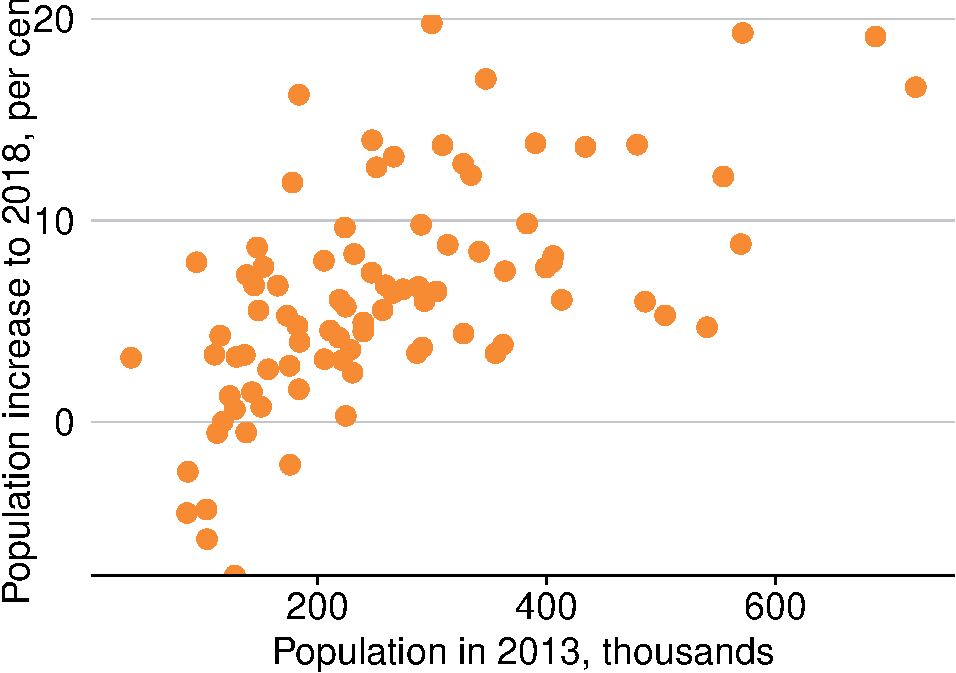
\includegraphics{Data_visualisation_files/figure-latex/scatter1-1.pdf}

It looks like the areas with the largest population grew the most between 2013 and 2018. To explore the relationship further, you can add a line-of-best-fit with \texttt{geom\_smooth}:

\begin{Shaded}
\begin{Highlighting}[]
\NormalTok{population_diff }\OperatorTok\StringTok{ }
\StringTok{        }\KeywordTok{ggplot}\NormalTok{(}\KeywordTok{aes}\NormalTok{(}\DataTypeTok{x =}\NormalTok{ y2013}\OperatorTok{/}\DecValTok{1000}\NormalTok{,  }\CommentTok{# display the x-axis as thousands}
                   \DataTypeTok{y =}\NormalTok{ pop_change)) }\OperatorTok{+}
\StringTok{        }\KeywordTok{geom_point}\NormalTok{(}\DataTypeTok{size =} \DecValTok{4}\NormalTok{) }\OperatorTok{+}\StringTok{ }
\StringTok{        }\KeywordTok{geom_smooth}\NormalTok{() }\OperatorTok{+}\StringTok{ }
\StringTok{        }\KeywordTok{geom_hline}\NormalTok{(}\DataTypeTok{yintercept =} \DecValTok{0}\NormalTok{) }\OperatorTok{+}
\StringTok{        }\KeywordTok{theme_grattan}\NormalTok{() }\OperatorTok{+}
\StringTok{        }\KeywordTok{theme}\NormalTok{(}\DataTypeTok{axis.title.y =} \KeywordTok{element_text}\NormalTok{(}\DataTypeTok{angle =} \DecValTok{90}\NormalTok{)) }\OperatorTok{+}
\StringTok{        }\KeywordTok{grattan_y_continuous}\NormalTok{() }\OperatorTok{+}\StringTok{ }
\StringTok{        }\KeywordTok{labs}\NormalTok{(}\DataTypeTok{y =} \StringTok{"Population increase to 2018, per cent"}\NormalTok{,}
             \DataTypeTok{x =} \StringTok{"Population in 2013, thousands"}\NormalTok{)}
\end{Highlighting}
\end{Shaded}

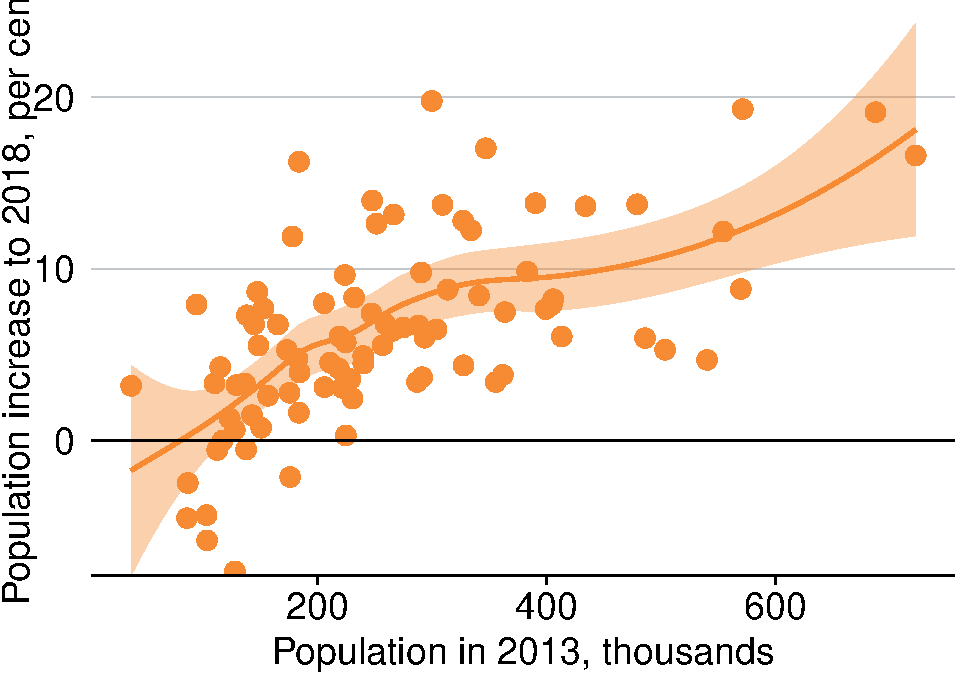
\includegraphics{Data_visualisation_files/figure-latex/scatter2-1.pdf}

You could colour-code positive and negative changes from within the \texttt{geom\_point} aesthetic. Making a change there won't pass through to the \texttt{geom\_smooth} aesthetic, so your line-of-best-fit will apply to all data points.

\begin{Shaded}
\begin{Highlighting}[]
\NormalTok{population_diff }\OperatorTok\StringTok{ }
\StringTok{        }\KeywordTok{ggplot}\NormalTok{(}\KeywordTok{aes}\NormalTok{(}\DataTypeTok{x =}\NormalTok{ y2013}\OperatorTok{/}\DecValTok{1000}\NormalTok{,  }\CommentTok{# display the x-axis as thousands}
                   \DataTypeTok{y =}\NormalTok{ pop_change)) }\OperatorTok{+}
\StringTok{        }\KeywordTok{geom_point}\NormalTok{(}\KeywordTok{aes}\NormalTok{(}\DataTypeTok{colour =}\NormalTok{ pop_change }\OperatorTok{<}\StringTok{ }\DecValTok{0}\NormalTok{),}
                   \DataTypeTok{size =} \DecValTok{4}\NormalTok{) }\OperatorTok{+}\StringTok{ }
\StringTok{        }\KeywordTok{geom_smooth}\NormalTok{() }\OperatorTok{+}\StringTok{ }
\StringTok{        }\KeywordTok{geom_hline}\NormalTok{(}\DataTypeTok{yintercept =} \DecValTok{0}\NormalTok{) }\OperatorTok{+}
\StringTok{        }\KeywordTok{theme_grattan}\NormalTok{() }\OperatorTok{+}
\StringTok{        }\KeywordTok{theme}\NormalTok{(}\DataTypeTok{axis.title.y =} \KeywordTok{element_text}\NormalTok{(}\DataTypeTok{angle =} \DecValTok{90}\NormalTok{)) }\OperatorTok{+}
\StringTok{        }\KeywordTok{grattan_y_continuous}\NormalTok{() }\OperatorTok{+}\StringTok{ }
\StringTok{        }\KeywordTok{grattan_colour_manual}\NormalTok{(}\DecValTok{2}\NormalTok{) }\OperatorTok{+}
\StringTok{        }\KeywordTok{labs}\NormalTok{(}\DataTypeTok{y =} \StringTok{"Population increase to 2018, per cent"}\NormalTok{,}
             \DataTypeTok{x =} \StringTok{"Population in 2013, thousands"}\NormalTok{)}
\end{Highlighting}
\end{Shaded}

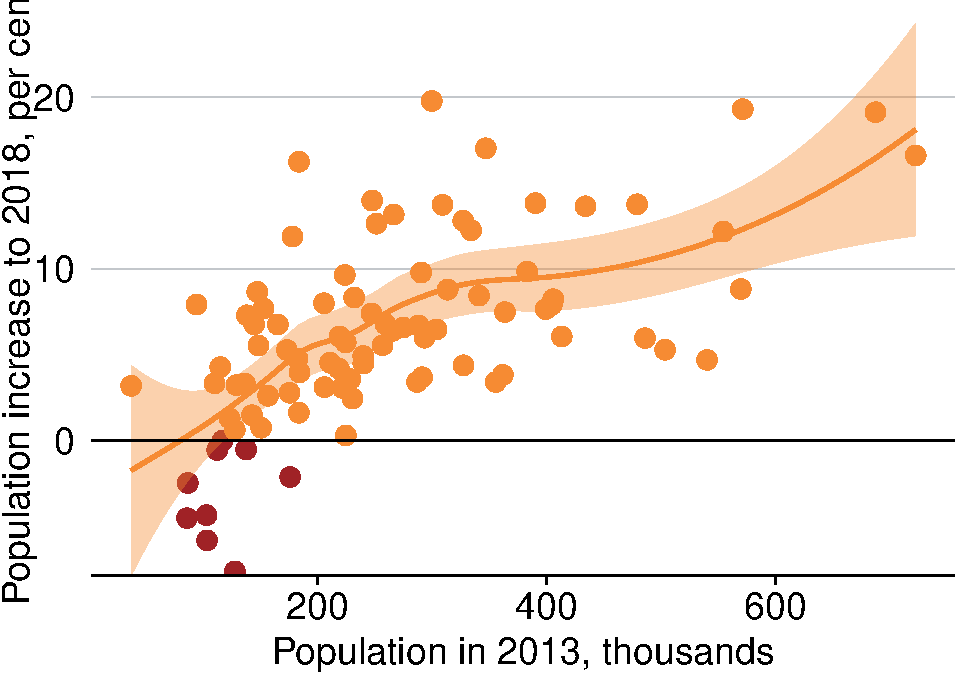
\includegraphics{Data_visualisation_files/figure-latex/scatter3-1.pdf}

Like the charts above, you could facet this by state to see if there were any interesting patterns. We'll filter out ACT and NT because they only have one and two data points (SA4s) in them, respectively.

\begin{Shaded}
\begin{Highlighting}[]
\NormalTok{population_diff }\OperatorTok\StringTok{ }
\StringTok{        }\KeywordTok{filter}\NormalTok{(state }\OperatorTok{!=}\StringTok{ "ACT"}\NormalTok{,}
\NormalTok{               state }\OperatorTok{!=}\StringTok{ "NT"}\NormalTok{) }\OperatorTok\StringTok{ }
\StringTok{        }\KeywordTok{ggplot}\NormalTok{(}\KeywordTok{aes}\NormalTok{(}\DataTypeTok{x =}\NormalTok{ y2013}\OperatorTok{/}\DecValTok{1000}\NormalTok{,  }\CommentTok{# display the x-axis as thousands}
                   \DataTypeTok{y =}\NormalTok{ pop_change)) }\OperatorTok{+}
\StringTok{        }\KeywordTok{geom_point}\NormalTok{(}\KeywordTok{aes}\NormalTok{(}\DataTypeTok{colour =}\NormalTok{ pop_change }\OperatorTok{<}\StringTok{ }\DecValTok{0}\NormalTok{),}
                   \DataTypeTok{size =} \DecValTok{2}\NormalTok{) }\OperatorTok{+}
\StringTok{        }\KeywordTok{geom_smooth}\NormalTok{() }\OperatorTok{+}\StringTok{ }
\StringTok{        }\KeywordTok{geom_hline}\NormalTok{(}\DataTypeTok{yintercept =} \DecValTok{0}\NormalTok{) }\OperatorTok{+}
\StringTok{        }\KeywordTok{theme_grattan}\NormalTok{() }\OperatorTok{+}
\StringTok{        }\KeywordTok{theme}\NormalTok{(}\DataTypeTok{axis.title.y =} \KeywordTok{element_text}\NormalTok{(}\DataTypeTok{angle =} \DecValTok{90}\NormalTok{)) }\OperatorTok{+}
\StringTok{        }\KeywordTok{grattan_y_continuous}\NormalTok{() }\OperatorTok{+}\StringTok{ }
\StringTok{        }\KeywordTok{grattan_colour_manual}\NormalTok{(}\DecValTok{2}\NormalTok{) }\OperatorTok{+}
\StringTok{        }\KeywordTok{labs}\NormalTok{(}\DataTypeTok{y =} \StringTok{"Population increase to 2018, per cent"}\NormalTok{,}
             \DataTypeTok{x =} \StringTok{"Population in 2013, thousands"}\NormalTok{) }\OperatorTok{+}
\StringTok{        }\KeywordTok{facet_wrap}\NormalTok{(state }\OperatorTok{~}\StringTok{ }\NormalTok{.)}
\end{Highlighting}
\end{Shaded}

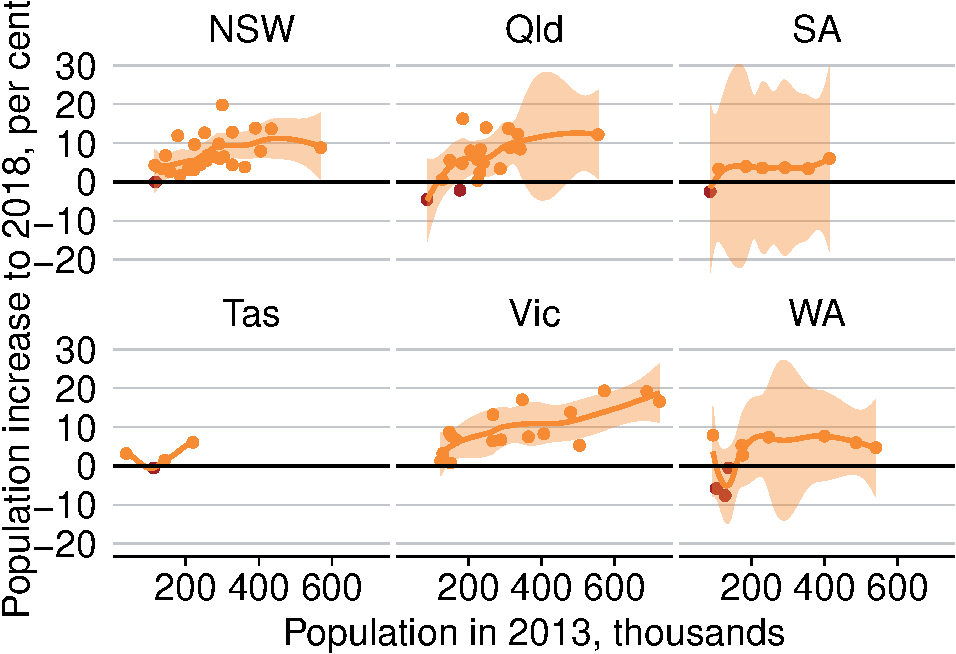
\includegraphics{Data_visualisation_files/figure-latex/scatter4-1.pdf}

\hypertarget{distributions}{%
\subsection{Distributions}\label{distributions}}

\texttt{geom\_histogram}
\texttt{geom\_density}

\texttt{ggridges::}

\hypertarget{maps}{%
\subsection{Maps}\label{maps}}

\hypertarget{sf-objects}{%
\subsubsection{\texorpdfstring{\texttt{sf} objects}{sf objects}}\label{sf-objects}}

{[}what is{]}

\hypertarget{using-absmapsdata}{%
\subsubsection{\texorpdfstring{Using \texttt{absmapsdata}}{Using absmapsdata}}\label{using-absmapsdata}}

The \texttt{absmapsdata} contains compressed, and tidied \texttt{sf} objects containing geometric information about ABS data structures. The included objects are:

\begin{itemize}
\tightlist
\item
  Statistical Area 1 2011: \texttt{sa12011}
\item
  Statistical Area 1 2016: \texttt{sa12016}
\item
  Statistical Area 2 2011: \texttt{sa22011}
\item
  Statistical Area 2 2016: \texttt{sa22016}
\item
  Statistical Area 3 2011: \texttt{sa32011}
\item
  Statistical Area 3 2016: \texttt{sa32016}
\item
  Statistical Area 4 2011: \texttt{sa42011}
\item
  Statistical Area 4 2016: \texttt{sa42016}
\item
  Greater Capital Cities 2011: \texttt{gcc2011}
\item
  Greater Capital Cities 2016: \texttt{gcc2016}
\item
  Remoteness Areas 2011: \texttt{ra2011}
\item
  Remoteness Areas 2016: \texttt{ra2016}
\item
  State 2011: \texttt{state2011}
\item
  State 2016: \texttt{state2016}
\item
  Commonwealth Electoral Divisions 2018: \texttt{ced2018}
\item
  State Electoral Divisions 2018:\texttt{sed2018}
\item
  Local Government Areas 2016: \texttt{lga2016}
\item
  Local Government Areas 2018: \texttt{lga2018}
\end{itemize}

You can install the package from Github. You will also need the \texttt{sf} package installed to handle the \texttt{sf} objects.

\begin{Shaded}
\begin{Highlighting}[]
\NormalTok{devtools}\OperatorTok{::}\KeywordTok{install_github}\NormalTok{(}\StringTok{"wfmackey/absmapsdata"}\NormalTok{)}
\KeywordTok{library}\NormalTok{(absmapsdata)}

\KeywordTok{install.packages}\NormalTok{(}\StringTok{"sf"}\NormalTok{)}
\KeywordTok{library}\NormalTok{(sf)}
\end{Highlighting}
\end{Shaded}

\hypertarget{making-choropleth-maps}{%
\subsubsection{Making choropleth maps}\label{making-choropleth-maps}}

Choropleth maps break an area into `bits', and colours each `bit' according to a variable.

SA4 is the largest non-state statistical area in the ABS ASGS standard.

You can join the \texttt{sf} objects from \texttt{absmapsdata} to your dataset using \texttt{left\_join}. The variable names might be different -- eg \texttt{sa4\_name} compared to \texttt{sa4\_name\_2016} -- so use the \texttt{by} function to match them.

\begin{Shaded}
\begin{Highlighting}[]
\NormalTok{map_data <-}\StringTok{ }\NormalTok{population_diff }\OperatorTok\StringTok{ }
\StringTok{        }\KeywordTok{left_join}\NormalTok{(sa42016, }\DataTypeTok{by =} \KeywordTok{c}\NormalTok{(}\StringTok{"sa4_name"}\NormalTok{ =}\StringTok{ "sa4_name_2016"}\NormalTok{))}

\KeywordTok{head}\NormalTok{(map_data }\OperatorTok\StringTok{ }
\StringTok{       }\KeywordTok{select}\NormalTok{(sa4_name, geometry))}
\end{Highlighting}
\end{Shaded}

\begin{verbatim}
## # A tibble: 6 x 3
## # Groups:   state [2]
##   state sa4_name                                                   geometry
##   <chr> <chr>                                            <MULTIPOLYGON [°]>
## 1 ACT   Australian Capita~ (((148.8041 -35.71402, 148.8018 -35.7121, 148.7~
## 2 NSW   Capital Region     (((150.3113 -35.66588, 150.3126 -35.66814, 150.~
## 3 NSW   Central Coast      (((151.315 -33.55582, 151.3159 -33.55503, 151.3~
## 4 NSW   Central West       (((150.6107 -33.06614, 150.6117 -33.07051, 150.~
## 5 NSW   Coffs Harbour - G~ (((153.2785 -29.91874, 153.2773 -29.92067, 153.~
## 6 NSW   Far West and Orana (((150.1106 -31.74613, 150.1103 -31.74892, 150.~
\end{verbatim}

You then plot a map like you would any other \texttt{ggplot}: provide your data, choose your \texttt{aes} and your \texttt{geom}. For maps with \texttt{sf} objects, the key \textbf{aesthetic} is \texttt{geometry\ =\ geometry}, and the \textbf{geom} is \texttt{geom\_sf}.

\begin{Shaded}
\begin{Highlighting}[]
\NormalTok{map <-}\StringTok{ }\NormalTok{map_data }\OperatorTok\StringTok{ }
\StringTok{        }\KeywordTok{ggplot}\NormalTok{(}\KeywordTok{aes}\NormalTok{(}\DataTypeTok{geometry =}\NormalTok{ geometry,}
                   \DataTypeTok{fill =}\NormalTok{ pop_change)) }\OperatorTok{+}
\StringTok{        }\KeywordTok{geom_sf}\NormalTok{(}\DataTypeTok{lwd =} \DecValTok{0}\NormalTok{) }\OperatorTok{+}
\StringTok{        }\KeywordTok{theme_void}\NormalTok{() }\OperatorTok{+}
\StringTok{        }\KeywordTok{grattan_fill_manual}\NormalTok{(}\DataTypeTok{discrete =} \OtherTok{FALSE}\NormalTok{, }
                            \DataTypeTok{palette =} \StringTok{"diverging"}\NormalTok{,}
                            \DataTypeTok{limits =} \KeywordTok{c}\NormalTok{(}\OperatorTok{-}\DecValTok{20}\NormalTok{, }\DecValTok{20}\NormalTok{),}
                            \DataTypeTok{breaks =} \KeywordTok{seq}\NormalTok{(}\OperatorTok{-}\DecValTok{20}\NormalTok{, }\DecValTok{20}\NormalTok{, }\DecValTok{10}\NormalTok{)) }\OperatorTok{+}
\StringTok{  }\KeywordTok{labs}\NormalTok{(}\DataTypeTok{fill =} \StringTok{"Population change"}\NormalTok{)}

\NormalTok{map}
\end{Highlighting}
\end{Shaded}

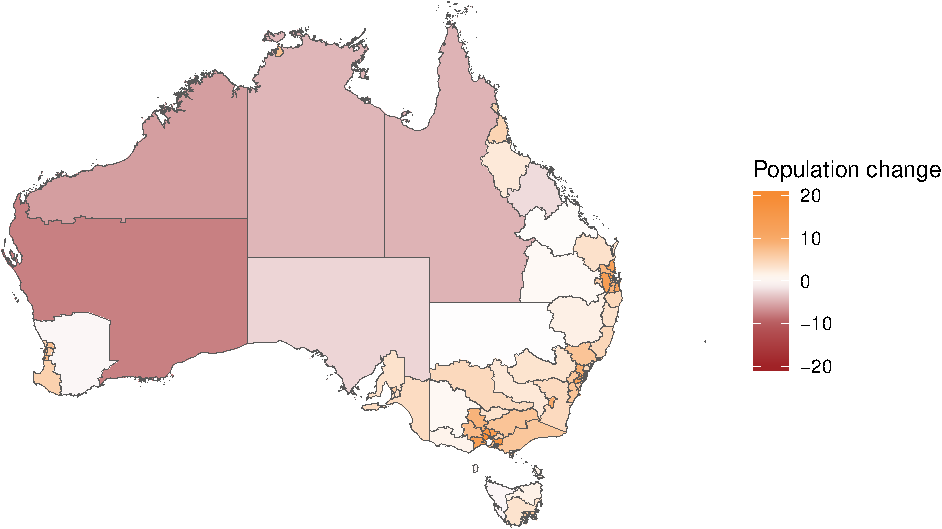
\includegraphics{Data_visualisation_files/figure-latex/map1-1.pdf}

\hypertarget{creating-simple-interactive-graphs-with-plotly}{%
\section{\texorpdfstring{Creating simple interactive graphs with \texttt{plotly}}{Creating simple interactive graphs with plotly}}\label{creating-simple-interactive-graphs-with-plotly}}

\texttt{plotly::ggplotly()}

\hypertarget{bin-generate-data-used-before-prior-sections-are-constructed}{%
\section{bin: generate data used (before prior sections are constructed)}\label{bin-generate-data-used-before-prior-sections-are-constructed}}

\begin{Shaded}
\begin{Highlighting}[]
\KeywordTok{library}\NormalTok{(tidyverse)}
\KeywordTok{library}\NormalTok{(janitor)}
\KeywordTok{library}\NormalTok{(absmapsdata)}

\NormalTok{data <-}\StringTok{ }\KeywordTok{read_csv}\NormalTok{(}\StringTok{"data/ABS_REGIONAL_ASGS2016_02082019164509969.csv"}\NormalTok{) }\OperatorTok\StringTok{ }
\StringTok{        }\KeywordTok{clean_names}\NormalTok{() }\OperatorTok\StringTok{ }
\StringTok{        }\KeywordTok{select}\NormalTok{(}\DataTypeTok{data_code =}\NormalTok{ measure,}
\NormalTok{               data_item,}
               \DataTypeTok{asgs =}\NormalTok{ regiontype,}
               \DataTypeTok{sa4_code_2016 =}\NormalTok{ asgs_}\DecValTok{2016}\NormalTok{,}
               \DataTypeTok{sa4_name_2016 =}\NormalTok{ region,}
               \DataTypeTok{year =}\NormalTok{ time,}
\NormalTok{               value) }\OperatorTok\StringTok{ }
\StringTok{        }\KeywordTok{mutate}\NormalTok{(}\DataTypeTok{sa4_code_2016 =} \KeywordTok{as.character}\NormalTok{(sa4_code_}\DecValTok{2016}\NormalTok{)) }\OperatorTok\StringTok{ }
\StringTok{        }\KeywordTok{left_join}\NormalTok{(sa42016 }\OperatorTok\StringTok{ }\KeywordTok{select}\NormalTok{(sa4_code_}\DecValTok{2016}\NormalTok{, state_name_}\DecValTok{2016}\NormalTok{)) }\OperatorTok\StringTok{ }
\StringTok{        }\KeywordTok{rename}\NormalTok{(}\DataTypeTok{state =}\NormalTok{ state_name_}\DecValTok{2016}\NormalTok{,}
               \DataTypeTok{sa4_code =}\NormalTok{ sa4_code_}\DecValTok{2016}\NormalTok{,}
               \DataTypeTok{sa4_name =}\NormalTok{ sa4_name_}\DecValTok{2016}\NormalTok{) }\OperatorTok\StringTok{ }
\StringTok{        }\KeywordTok{mutate}\NormalTok{(}\DataTypeTok{state_long =}\NormalTok{ state,}
               \DataTypeTok{state =}\NormalTok{ strayr}\OperatorTok{::}\KeywordTok{strayr}\NormalTok{(state_long))}
               
\KeywordTok{write_csv}\NormalTok{(data, }\StringTok{"data/population_sa4.csv"}\NormalTok{)}
\end{Highlighting}
\end{Shaded}

\hypertarget{reading-data}{%
\chapter{Reading data}\label{reading-data}}

\hypertarget{importing-data}{%
\section{Importing data}\label{importing-data}}

\hypertarget{reading-csv-files}{%
\subsection{Reading CSV files}\label{reading-csv-files}}

\hypertarget{read_csv}{%
\subsubsection{\texorpdfstring{\texttt{read\_csv()}}{read\_csv()}}\label{read_csv}}

The \texttt{read\_csv()} function from the \texttt{tidyverse} is quicker and smarter than \texttt{read.csv} in base R.

Pitfalls:
1. read\_csv is quicker because it surveys a sample of the data

We can also compress \texttt{.csv} files into \texttt{.zip} files and read them \emph{directly} using \texttt{read\_csv()}:

\begin{Shaded}
\begin{Highlighting}[]
\KeywordTok{read_csv}\NormalTok{(}\StringTok{"data/my_data.zip"}\NormalTok{)}
\end{Highlighting}
\end{Shaded}

This is useful for two reasons:

\begin{enumerate}
\def\labelenumi{\arabic{enumi}.}
\tightlist
\item
  The data takes up less room on your computer; and
\item
  The original data, which shouldn't ever be directly edited, is protected and cannot be directly edited.
\end{enumerate}

\hypertarget{data.tablefread}{%
\subsubsection{\texorpdfstring{\texttt{data.table::fread()}}{data.table::fread()}}\label{data.tablefread}}

The \texttt{fread} function from \texttt{data.table} is quicker than both \texttt{read.csv} and \texttt{read\_csv}.

\hypertarget{readxlread_excel}{%
\subsection{\texorpdfstring{\texttt{readxl::read\_excel()}}{readxl::read\_excel()}}\label{readxlread_excel}}

\hypertarget{rio}{%
\subsection{\texorpdfstring{\texttt{rio}}{rio}}\label{rio}}

\hypertarget{readabs}{%
\subsection{\texorpdfstring{\texttt{readabs}}{readabs}}\label{readabs}}

\hypertarget{reading-common-files}{%
\section{Reading common files:}\label{reading-common-files}}

\begin{itemize}
\tightlist
\item
  TableBuilder CSVSTRINGs
\item
  HES household file
\item
  SIH
\item
  LSAY and derivatives
\end{itemize}

See data directory for a list of microdata available to Grattan.

\hypertarget{appropriately-renaming-variables}{%
\section{Appropriately renaming variables}\label{appropriately-renaming-variables}}

As shown in the style guide

Add \texttt{rename\_abs} function to a common Grattan package?

\hypertarget{getting-to-tidy-data}{%
\section{Getting to tidy data}\label{getting-to-tidy-data}}

\texttt{pivot\_long()} and \texttt{pivot\_wide()}
\emph{Make sure these are stable btw}

\hypertarget{different-data-types}{%
\chapter{Different data types}\label{different-data-types}}

\hypertarget{tidy-data}{%
\section{Tidy data}\label{tidy-data}}

Other data structures

\hypertarget{dates-with-lubridate}{%
\section{\texorpdfstring{Dates with \texttt{lubridate::}}{Dates with lubridate::}}\label{dates-with-lubridate}}

The \texttt{lubridate::} package

\hypertarget{strings-with-stringr}{%
\section{\texorpdfstring{Strings with \texttt{stringr::}}{Strings with stringr::}}\label{strings-with-stringr}}

\begin{itemize}
\tightlist
\item
  Replacing values
\item
  Matching values
\item
  Separating columns
\end{itemize}

\hypertarget{factors-with-forcats}{%
\section{\texorpdfstring{Factors with \texttt{forcats::}}{Factors with forcats::}}\label{factors-with-forcats}}

\begin{itemize}
\tightlist
\item
  Dangers with factors
\end{itemize}

\hypertarget{data-transformation}{%
\chapter{Data transformation}\label{data-transformation}}

\hypertarget{the-pipe}{%
\section{The pipe}\label{the-pipe}}

\hypertarget{key-dplyr-functions}{%
\section{\texorpdfstring{Key \texttt{dplyr} functions:}{Key dplyr functions:}}\label{key-dplyr-functions}}

All have the same syntax structure, which enable pipe-chains.

\hypertarget{filter-with-filter}{%
\section{\texorpdfstring{Filter with \texttt{filter()}}{Filter with filter()}}\label{filter-with-filter}}

\hypertarget{arrange-with-arrange}{%
\section{\texorpdfstring{Arrange with \texttt{arrange()}}{Arrange with arrange()}}\label{arrange-with-arrange}}

\hypertarget{select-variables-with-select}{%
\section{\texorpdfstring{Select variables with \texttt{select()}}{Select variables with select()}}\label{select-variables-with-select}}

\hypertarget{group-data-with-group_by}{%
\section{\texorpdfstring{Group data with \texttt{group\_by()}}{Group data with group\_by()}}\label{group-data-with-group_by}}

\hypertarget{edit-and-add-new-variables-with-mutate}{%
\section{\texorpdfstring{Edit and add new variables with \texttt{mutate()}}{Edit and add new variables with mutate()}}\label{edit-and-add-new-variables-with-mutate}}

\hypertarget{cases-when-you-should-use-case_when}{%
\subsection{\texorpdfstring{Cases when you should use \texttt{case\_when()}}{Cases when you should use case\_when()}}\label{cases-when-you-should-use-case_when}}

\hypertarget{summarise-data-with-summarise}{%
\section{\texorpdfstring{Summarise data with \texttt{summarise()}}{Summarise data with summarise()}}\label{summarise-data-with-summarise}}

\hypertarget{joining-datasets-with-_join}{%
\section{\texorpdfstring{Joining datasets with \texttt{*\_join()}}{Joining datasets with *\_join()}}\label{joining-datasets-with-_join}}

\hypertarget{analysis}{%
\chapter{Analysis}\label{analysis}}

\hypertarget{creating-functions}{%
\chapter{Creating functions}\label{creating-functions}}

\hypertarget{it-can-be-useful-to-make-your-own-function}{%
\section{It can be useful to make your own function}\label{it-can-be-useful-to-make-your-own-function}}

Why on earth would you create your own function?

\hypertarget{defining-simple-functions}{%
\section{Defining simple functions}\label{defining-simple-functions}}

\hypertarget{more-complex-functions}{%
\section{More complex functions}\label{more-complex-functions}}

\hypertarget{sets-of-functions}{%
\section{Sets of functions}\label{sets-of-functions}}

\hypertarget{using-purrrmap}{%
\section{\texorpdfstring{Using \texttt{purrr::map}}{Using purrr::map}}\label{using-purrrmap}}

\hypertarget{sharing-your-useful-functions-with-grattan}{%
\section{Sharing your useful functions with Grattan}\label{sharing-your-useful-functions-with-grattan}}

\hypertarget{version-control}{%
\chapter{Version control}\label{version-control}}

\hypertarget{version-control-is-important-and-intimidating}{%
\section{Version control is important and intimidating}\label{version-control-is-important-and-intimidating}}

Version control is great!

\hypertarget{github}{%
\section{Github}\label{github}}

We use Github to version-control and share reports in LaTeX, so you're already a bit set-up.

\hypertarget{git}{%
\section{Git}\label{git}}

Using Git within R Studio\ldots{}

\bibliography{book.bib,packages.bib}


\end{document}
